\documentclass[12 pt,a4paper]{report}
\usepackage[utf8]{vietnam}
\usepackage{ucs}
\usepackage{amsmath}
\usepackage{amsfonts}
\usepackage{amssymb}
\usepackage{graphicx}
\usepackage{titlesec}
\usepackage{amssymb}
\usepackage{algorithm}
\usepackage{algpseudocode}
\usepackage{xr}
\usepackage{microtype}
\usepackage{sectsty}
\usepackage{subfigure}
\usepackage[subfigure]{tocloft}
%\usepackage{caption}
%\usepackage{subcaption}
\usepackage[left=3.5 cm,right=2 cm,top=2.54 cm,bottom=2.54 cm]{geometry}
%bia

%het bia
\setlength{\parskip}{0.5 em} % dan cach giua cac doan van
%\input setbmp
\usepackage[unicode]{hyperref} % tu dong tao bookmark
\usepackage{tocloft,calc}
\chapternumberfont{\changefontsizes{20pt}}
\chaptertitlefont{\changefontsizes{30pt}}
\renewcommand{\cftchappresnum}{Chương }
\AtBeginDocument{\addtolength\cftchapnumwidth{\widthof{\bfseries {Chương } }}}
\renewcommand{\baselinestretch}{1.3} % dan dong
\setlength{\parindent}{5 ex} % dieu chinh tab moi dau doan van
%======================================
% header_footer
\usepackage{fancyhdr}
\pagestyle{fancy}
\usepackage{scrextend}
\fancyhf{}
% ============= package insert code =========================
\usepackage{listings}
\usepackage{color}
\definecolor{dkgreen}{rgb}{0,0.6,0}
\definecolor{gray}{rgb}{0.5,0.5,0.5}
\definecolor{mauve}{rgb}{0.58,0,0.82} 
\lstset{frame=tb,
  language=C++,
  aboveskip=3mm,
  belowskip=3mm,
  showstringspaces=false,
  columns=flexible,
  basicstyle={\small\ttfamily},
  numbers=none,
  numberstyle=\tiny\color{gray},
  keywordstyle=\color{blue},
  commentstyle=\color{dkgreen},
  stringstyle=\color{mauve},
  breaklines=true,
  breakatwhitespace=true,
  tabsize=3
}
%\setcounter{secnumdepth}{4} %đánh số subsubsection
% package table
\usepackage{array}
\usepackage{multirow}
\usepackage{longtable}
\usepackage{lipsum} % just for dummy text- not needed for a longtable
%======================================
\usepackage{subfiles} % bien dich tai file con, khong can phai quay ve main 
%\usepackage{subfig}
\usepackage{subfigure}
%cac goi danh cho phan thuat ngu viet tat
\usepackage{glossaries}
%dong khung phu luc
\usepackage{xcolor}
\usepackage{titlesec}
\usepackage{mdframed}
\usepackage{amsmath}
\usepackage{fancybox}%khung cho bia
\newmdenv[linecolor=black,skipabove=\topsep,skipbelow=\topsep,
leftmargin=-5pt,rightmargin=-5pt,
innerleftmargin=5pt,innerrightmargin=5pt]{mybox}
\def\dotfill#1{\cleaders\hbox to #1{.}\hfill}
\newcommand\dotline[2][.5em]{\leavevmode\hbox to #2{\dotfill{#1}\hfil}}
\begin{document}

\title{ĐỒ ÁN TỐT NGHIỆP 2018}
%\maketitle
\subfile{bia.tex}
\pagebreak
\subfile{bialot.tex}
\pagebreak
\pagenumbering{roman}
\subfile{nxGiangVien}
\pagebreak
\subfile{nxPhanBien}
\pagebreak
\changefontsizes{13 pt}
\subfile{Loinoidau.tex}
\pagebreak
\subfile{Tomtatbaocao.tex}
\pagebreak
\subfile{ABSTRACT.tex}
\pagebreak

\renewcommand{\contentsname}{Mục lục}
\addcontentsline{toc}{chapter}{Mục lục} \tableofcontents
\pagebreak

\renewcommand{\listfigurename}{\changefontsizes{30pt}{Danh mục hình vẽ}}
\addcontentsline{toc}{chapter}{Danh mục hình vẽ}\listoffigures
\pagebreak

\renewcommand{\listtablename}{\changefontsizes{30pt}{Danh mục bảng biểu}}
\addcontentsline{toc}{chapter}{Danh mục bảng biểu}\listoftables
\pagebreak

{\pagestyle{plain}
\subfile{Danhmuccacthuatnguviettat.tex}
\cleardoublepage}

%======================================
% header_footer
\rhead{\textsc{Đồ Án Tốt Nghiệp 2019}}
\rfoot{ \textbf{\thepage}|Page}
\lfoot{\textsc{LÊ BÁ TUẤN ANH}} % left foot
\renewcommand{\headrulewidth}{2 pt} % cho header
\renewcommand{\footrulewidth}{1 pt} % cho footer
\changefontsizes{13 pt}
\pagenumbering{arabic}
%=======================
% noi dung

\chapter{Đặt vấn đề}
\label{chapter1}
Trong chương \ref{chapter1}, em nêu ra những mục chính là: Lý do chọn đề tài, mục tiêu của đề tài, các phương pháp sử dụng trong đồ án và cuối cùng là kết luận.
\section{Tổng quan về đề tài}
Thương mại điện tử là một khái niệm mới. Mặc dù ra đời chưa lâu nhưng nó đã nhanh chóng khẳng định được vị thế của mình nhờ sức hấp dẫn cũng như trên đà khá ngoạn ngục. Cùng với sự phát triển chóng mặt của Internet, thương mại điện tử đang có những bước tiến rất nhanh với tốc độ ngày càng cao.
\par
Cuối những năm 1900, thương mại điện tử vẫn còn là một khái niệm khá mới mẻ ở Việt Nam. Nhưng dưới sức lan toả rộng khắp của thương mại điện tử, các công ty Việt Nam cũng đang từng bước làm quen với phương thức kinh doanh hiện đại này.  \textls[-5]{Một số dự án thương mại điện tử ở Việt Nam đang phát triển rất mạnh mẽ như:}
\begin{itemize}
\item	thegioididong.vn, chuỗi cửa hàng thegioididong.com được thành lập từ năm 2004 chuyên bán lẻ các sản phẩm kỹ thuật số di động bao gồm điện thoại di động, máy tính bảng, laptop và phụ kiện điện tử với gần 1000 siêu thị tại 64 tỉnh thành trên khắp Việt Nam. Thế giới di động đã xây dựng được một dịch vụ khách hàng khác biệt vượt trội với văn hoá “Đặt khách hàng làm trung tâm” trong mọi suy nghĩ và hành động của mình với tất cả các nhân viên của công ty. Với uy tín của mình, thế giới di động hiện nay đứng top 1 bán hàng trực tuyến uy tín chất lượng với các mặt hàng di động, máy tính xách tay và các sản phẩm công nghệ cao.
\item	lazada.vn, là một website mua sắm trực tuyến được thiết kế chuyên nghiệp, hiện đại. Lazada là trang web được nhiều người sử dụng nhất hiện nay tại Việt Nam. Tuy nhiên công ty chủ quản của Lazada không phải của Việt Nam mà là của công ty Singapore có chi nhánh tại Việt Nam. Lazada là công ty bán hàng trực tuyến lớn nhất tại khu vực Đông Nam Á với rất nhiều chi nhánh tại các nước lớn trong khu vực như Indonesia, Thailand, Philippines, Malaysia, Singapore. Tuy nhiên, Lazada không cung cấp tất cả các hàng hóa dịch vụ mà chủ yếu là tạo ra sàn giao dịch online cho các cửa hàng đăng ký bán hàng trên website, công ty chỉ đảm bảo về giao dịch trực tuyến và quản lý cửa hàng, khách hàng.
\item	tiki.vn, Tiki là một trong những trang web mua sắm trực tuyến hàng đầu Việt Nam sở hữu hơn 800.000 khách hàng và cung cấp đến 120.000 sản phẩm thuộc 10 ngành hàng khác nhau như: Sách, Làm đẹp – Sức khoẻ, Nhà cửa – Đời sống, Điện thoại – Máy tính bảng, Thiết bị số – Phụ kiện số, Điện gia dụng, Thiết bị văn phòng phẩm, Mẹ và Bé, Đồ chơi – Đồ lưu niệm, Thể thao – Dã ngoại với mức doanh số tăng trưởng gấp ba lần mỗi năm. Tiki.vn đã được trao tặng danh hiệu “website TMĐT được yêu thích năm 2014” do người tiêu dùng bình chọn sau 5 năm nỗ lực hoạt động không ngừng nghỉ. Mạng lưới giao hàng của TiKi phục vụ trên toàn quốc, miễn phí cho mọi đơn hàng từ 250.000đ, riêng tại TPHCM và Hà Nội chỉ từ 150.000đ. Dịch vụ vận chuyển trong 24h giúp khách hàng trải nghiệm mua sắm trực tuyến một cách tiện lợi vừa tiết kiệm được thời gian, công sức mà vẫn bảo đảm được các quyền lợi về bảo hành hay đổi/trả dễ dàng trong vòng 30 ngày.
\item sendo.vn, Là trang web mua bán trực tuyến của Tập đoàn FPT nhằm kết nối người mua và người bán trên toàn quốc. Ra đời là một dự án Thương mại Điện tử do Công ty CP Dịch vụ Trực tuyến FPT (FPT Online) xây dựng và phát triển, Sendo.vn chính thức ra mắt người dùng vào tháng 9/2012. Ngày 13/5/2014, Công ty CP Công nghệ Sen Đỏ được thành lập, trực thuộc Tập đoàn FPT, là công ty chủ quản của Sendo.vn.
\item robins.vn Zalora là trang web mua sắm thời trang quốc tế được đầu tư vào thị trường Việt Nam khá mạnh trong thời gian gần đây. Với sự uy tín cao và nguồn vốn đầu tư khá mạnh, Zalora không khó để chiếm lĩnh thị trường thời trang online tại Việt Nam. Zalora có một hệ thống mua hàng trực tuyến nhanh gọn, dễ dàng, thuận tiện và tiết kiệm thời gian cho khách hàng. Ở Zalora bạn có thể mua tất cả món hàng thời trang nào mà bạn cần.
\item vatgia.com, Khi truy cập chợ mua bán online www.vatgia.com, khách hàng dễ dàng tìm kiếm thông tin với hàng nghìn gian hàng và sản phẩm về điện tử, công nghiệp,xe cộ, xây dựng – nhà cửa,hay các dịch vụ và giải trí. Gian hàng được trình bày một cách khoa học, kết hợp với nhiều công cụ tìm kiếm tiện lợi, dễ dàng cho người tiêu dùng có thể tìm được sản phẩm như mong muốn, rẻ, chính xác và trong thời gian ngắn nhất. Bên cạnh đó, website thương mại điện tử này còn cung cấp cho người tiêu dùng công cụ bình chọn đánh giá chất lượng dịch vụ của người bán, không gian để nhiều người đóng góp ý kiến, trao đổi thông tin về sản phẩm để tìm được những sản phẩm dịch vụ có giá cả và chất lượng tốt nhất.
\item chotot.com, Chợ Tốt ra đời vào năm 2012, là một kênh rao vặt trung gian, kết nối người bán và người mua bằng những giao dịch đơn giản, tiện lợi, nhanh chóng và an toàn. Tại Chợ Tốt, người dùng dễ dàng mua bán mọi mặt hàng, dù đó là đồ cũ hay đồ mới. Các lĩnh vực như bất động sản, xe cộ, đồ dùng cá nhân, đồ điện tử,...\cite{1}
\end{itemize}
\par
Trong cuộc cách mạng công nghệ 4.0, các công nghệ thay nhau áp dụng vào thương mại để phục vụ đời sống hàng ngày cho con người, thương mại điện tử giúp cho các nhà quản lý một phần nào trong việc mang sản phẩm của mình đến với người sử dụng, cũng giúp cho người tiêu dùng không mất quá nhiều thời gian để có cho mình sản phẩm đúng theo nhu cầu sử dụng.
\section{Mục tiêu của đề tài}
Trên thực tế các cửa hàng vẫn bán hàng theo phương thức truyền thống người mua hàng phải đến tận nơi để xem mua hàng hoá, vào thời kì cách mạng công nghệ 4.0 chúng ta phải đưa công nghệ vào thương mại để xoá bỏ phương thức mua bán truyền thống này. Dựa vào các lý do trên em đưa ra yêu cầu đối với website thương mại điện tử như sau:
\begin{itemize}
\item Đối với người quản lý:
\begin{itemize}
\item Phân quyền theo từng chức năng đối với các cấp người sử dụng website.
\item Cho phép người quản trị có tất cả các quyền đối với hệ thống.
\item Quản lý sản phẩm theo các thuộc tính của sản phẩm: ảnh, số lượng, giá bán, màu sắc, giá bán sỉ, kích cỡ,...
\item Quản lý các danh mục sản phẩm để người quản lý có thể mở rộng mặt hàng.
\item Quản lý người vận chuyển hàng.
\item Quản lý các đơn hàng.
\item Xem doanh thu theo tháng, hay các chuỗi ngày.
\item Quản lý các quảng cáo, ảnh giao diện, thông tin khách hàng, địa chỉ liên hệ với cửa hàng.
\item Quản lý bài đăng cho website.
\end{itemize}
\item Đối với người tiêu dùng:
\begin{itemize}
\item Giao diện người dùng thân thiện với người dùng.
\item Hiển thị các danh mục sản phẩm để người dùng dễ chọn lựa.
\item Tìm kiếm theo gợi ý theo tên sản phẩm có trong hệ thống.
\item Hiển thị thông tin sản phầm rõ ràng và đầy đủ.
\item Giao diện thanh toán dễ dàng cho người mua hàng.
\item Đăng ký, đăng nhập cho người dùng để lưu thông tin vào đơn hàng giúp người quản lý dễ dàng giao hàng đến người tiêu dùng.
\item Chức năng quên mật khẩu để người dùng có thể lấy lại tài khoản và xem những đơn hàng mà người dùng đã mua ở website.
\end{itemize}
\end{itemize}
\section{Các phương pháp sử dụng trong thiết kế}
Các phương pháp mà em sử dụng gồm có:
\begin{itemize}
\item   Tham khảo tài liệu: tham khảo tài liệu từ sách báo về điện tử, từ mạng internet, kế thừa và phát triển các kết quả nghiên cứu đã có.
\item   Quan sát, học hỏi: thảo luận cùng thầy và các bạn để đưa ra được hướng đi tốt nhất, đạt hiệu quả cao.
\item   Thực hành và sửa lỗi: tiến hành viết code và sửa lỗi để đạt được kết quả tối ưu nhất.
\end{itemize}\par
\section{Kết luận}
Mục tiêu của đề tài này là xây dựng website thương mại điện tử để thay thế phương thức mua bán truyền thống. Để hoàn thành đề tài cần có  những kiến thức về phân tích thiết kế hướng đối tượng, quy trình kiểm thử phần mềm, quy trình thiết kế phần mềm, kiến thức về lập trình hướng đối tượng, và những kiến thức thực tế về thương mại điện tử em tìm hiểu được từ các trang web thực tế. Từ đây em có những kế hoạch cụ thể để hoàn thành mục tiêu đề ra và được em trình bày ở các chương sau.



\chapter{Cơ sở lý thuyết}
\label{chapter2}
Chương \ref{chapter2} em sẽ trình bày những kiến thức và các công cụ cần có để xây dựng một website mà em tìm hiểu được để phục vụ cho những vấn đề nêu ra ở chương \ref{chapter1}
\section{Ngôn ngữ lập trình C\# } \label{ngonngu} 
C\# là một ngôn ngữ lập trình hướng đối tượng được phát triển bởi Microsoft, là phần khởi đầu cho kế hoạch .NET của Microsoft. Tên của ngôn ngữ bao gồm ký tự thăng theo Microsoft nhưng theo ECMA là C\#, chỉ bao gồm dấu số thường. Microsoft phát triển C\# dựa trên C++ và Java. C\# được miêu tả là ngôn ngữ có được sự cân bằng giữa C++, Visual Basic, Delphi và Java.
\par
C\# được thiết kế chủ yếu bởi Anders Hejlsberg kiến trúc sư phần mềm nổi tiếng với các sản phẩm Turbo Pascal, Delphi, J++, WFC.
Tiêu chuẩn ECMA liệt kê các mục tiêu của việc thiết kế ngôn ngữ C\#:
\begin{itemize}
\item Ngôn ngữ được dự định là một ngôn ngữ lập trình đơn giản, hiện đại, hướng đến nhiều mục đích sử dụng, và là một ngôn ngữ lập trình hướng đối tượng.
\item Ngôn ngữ và việc triển khai đáp ứng các nguyên tắc của ngành kỹ thuật phần mềm như kiểm tra chặt chẽ kiểu dữ liệu, kiểm tra giới hạn mảng, phát hiện các trường hợp sử dụng các biến chưa có dữ liệu, và tự động thu gom rác. Tính mạnh mẽ, sự bền bỉ, và năng suất của việc lập trình là rất quan trọng đối với ngôn ngữ này.
\item Ngôn ngữ sẽ được sử dụng để phát triển các thành phần của phần mềm theo hướng thích hợp cho việc triển khai trong các môi trường phân tán.
\item Khả năng di chuyển (portability) là rất quan trọng, đặc biệt là đối với những lập trình viên đã quen với C và C++.
\item Hỗ trợ quốc tế hóa.
\item Ngôn ngữ sẽ được thiết kế để phù hợp với việc viết các ứng dụng cho cả hai hệ thống: hosted và nhúng, từ các phần mềm quy mô lớn, đến các phần mềm chỉ có các chức năng đơn giản.
\item Mặc dù các ứng dụng C\# có tính kinh tế đối với các yêu cầu về bộ nhớ và chế độ xử lý, ngôn ngữ này không cạnh tranh trực tiếp về hiệu năng và kích thước đối với ngôn ngữ C hoặc assembly
\item C\# được biên dịch ra mã trung gian MSIL sau đó thực thi bởi Common Language Runtime (CLR) \cite{2}.
\end{itemize}
\par
Em chọn ngôn ngữ C\# bởi vì:
\begin{itemize}
\item Rất phổ biến và được sử dụng bởi hàng triệu lập trình viên trên toàn thế giới.
\item Dễ học và sử dụng.
\item So với Java thì nó là đối thủ lớn nhất. Chúng ta không so sánh 2 ngôn ngữ nhưng em thích C\# vì nó luôn cải tiến.
\item Nền tảng .NET cũng luôn phát triển ngày càng hiện đại trong khi Java phát triển chậm.
\end{itemize}

\section{.NET}
.NET bao gồm 3 thành phần:
\begin{itemize}
\item Runtime
\item Libraries
\item Toolings
\end{itemize}
\par
Quy trình biên dịch và chạy chương trình của .NET. Hình \ref{refhinh2_2} ta thấy từ source code qua trình biên dịch tương ứng của ngôn ngữ đấy trong hệ sinh thái .NET ví dụ như C\# compiler hay VB.NET compiler để sinh ra MSIL code.  Ngôn ngữ trung gian trong .NET nó khá gần với mã máy nhưng không chứa thông tin cụ thể về CPU, nên ngôn ngữ MSIL giúp cho đoạn code trung gian của chúng ta có thể hoạt động trên nhiều loại CPU (64bit, 32bit), cũng như nhiều loại kiến trúc khác nhau (ARM, Intel…). Trên thực tế một vài ngôn ngữ (Javascript, Python…) không sử dụng đến ngôn ngữ trung gian: Source sẽ được dịch thẳng ra mã máy tại ‘Runtime’. Điểm lợi của việc này là quá trình build được đơn giản hóa, tuy nhiên hiệu năng sẽ bị hạn chế.
Ngoài việc biên dịch, môi trường hoạt động (Runtime) còn có những công dụng như:
\begin{itemize}
\item Tự động quản lý bộ nhớ. Khi làm việc với những ngôn ngữ bậc cao như C\# hay Java, chúng ta không cần  giải phóng bộ nhớ bằng cách gọi free() như khi làm việc với C/C++. CLR bao gồm một công cụ dọn rác (Garbage collector -GC) sẽ tự động giải phóng những phần bộ nhớ không được sử dụng
\item Strong typings: CLR quản lý thông tin về các kiểu dữ liệu đã sử dụng. Điều này giúp cho lập trình viên có thể phân biệt được các định dạng thông tin của từng biến khác nhau (class, structure…)
\end{itemize}
\par
Khi làm việc với .NET, code của chúng ta sẽ tương tác với rất nhiều các class khác nhau. Tất cả những class này được định nghĩa trong hệ thống thư viện cơ bản của .NET được gọi tắt là BCL (Base class libraries). Mã nguồn của BCL, trái với mọi người hay nghĩ, là mã nguồn mở. Chúng ta có thể truy cập mã nguồn này tại sourceof.net. Các công cụ (toolings) của .NET bao gồm compiler và Visual Studio .NET sử dụng hệ thống build của Microsoft gọi là MSBuild. Đối với nền tảng .NET core mới thì chúng ta còn có thêm công cụ dòng lệnh (dotnet cli).
\begin{center}
    \begin{figure}[h]
    \begin{center}
     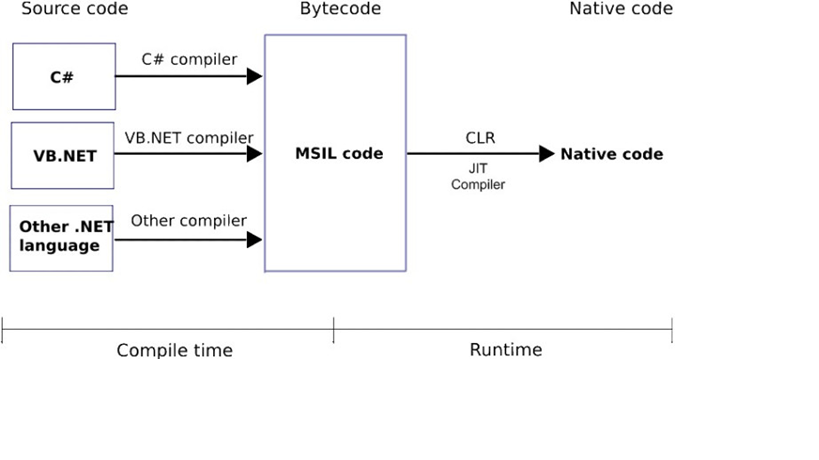
\includegraphics[scale=0.6]{image/chayDotNet.png}
    \end{center}
    \caption{Quy trình biên dịch và chạy chương trình}
    \label{refhinh2_2}
    \end{figure}
\end{center}
\par
Hình \ref{refhinh2_3} chúng ta có thể thấy về cơ bản, .NET Framework, .NET core và Mono là ba phiên bản .NET khác nhau (có nghĩa là mỗi phiên bản có Runtime, Libraries và Toolings riêng).
\begin{center}
    \begin{figure}[h]
    \begin{center}
     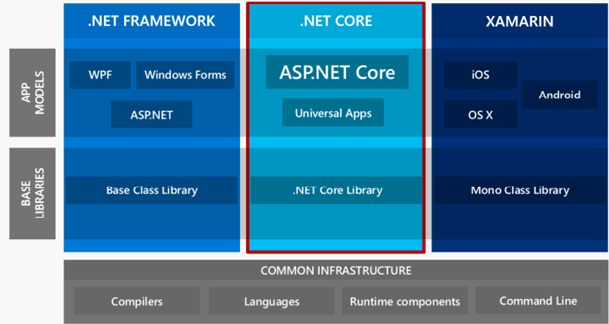
\includegraphics[scale=0.9]{image/kienTrucDotNetCore.png}
    \end{center}
    \caption{Kiến trúc của .NET }
    \label{refhinh2_3}
    \end{figure}
\end{center}
\begin{itemize}
\item .NET Framework được Microsoft đưa ra chính thức từ năm 2002. .NET Framework chỉ hoạt động trên Windows. Những nền tảng ứng dụng như WPF, Winforms, ASP.NET(1-4) hoạt động dựa trên .NET Framework.
\item Mono là phiên bản cộng đồng nhằm mang .NET đến những nền tảng ngoài Windows. Mono được phát triển chủ yếu nhằm xây dựng những ứng dụng với giao diện người dùng và được sử dụng rất rộng rãi: Unity Game, Xamarin…
\item Cho đến năm 2013, Microsoft định hướng đi đa nền tảng và phát triển .NET core. .NET core hiện được sử dụng trong các ứng dụng Universal Windows platform và ASP.NET Core.
\item Tuyệt đối không nên dùng Mono để vận hành webserver. Bộ máy dọn rác của Mono không được thiết kế để hoạt động với webserver và sẽ gây ra quá tải nhanh chóng
\item Nên lựa chọn .NET Framework hay .NET Core cho các web server .NET Core chạy được đa nền tảng và có hiệu năng cao hơn. Nhược điểm duy nhất của nó là số lượng thư viện hỗ trợ vẫn còn hạn chế. .NET Framework có hệ sinh thái lớn hơn với nhiều các thư viện hỗ trợ hơn.
\end{itemize}

\subsection{.NET Framework}
Như đã nêu ở phần \ref{ngonngu} ngôn ngữ C\# ra đời để phục vụ Microsoft phát triển nền tảng .NET Framework phục vụ phát triển cho nhiều ứng dụng cho nên C\# không đứng riêng lẻ mà nó là 1 phần của nền tảng .NET, .NET Framework bao gồm môi trường phát triển, hỗ trợ đa ngôn ngữ mà C\# là một trong số đó (ngoài ra có F\#, VB.NET, Managed C++, J\#).
Những thành phần của .NET Framework (Hình \ref{refhinh2_1}) bao gồm:
\begin{itemize}
\item Các ngôn ngữ lập trình .NET (C\#, VB.NET…).
\item Môi trường thực thi code (CLR) sẽ thực thi chương trình được viết từ ngôn ngữ lập trình.
\item Các công cụ phát triển như trình biên dịch CSC dùng để biên dịch ngôn ngữ C\# sang mã trung gian (MSIL) mà CLR có thể hiểu.
\item Tập các thư viện chuẩn (Class Library) như ADO.NET cho phép truy cập database (ví dụ SQL Server hoặc MySQL) và WCF cho phép tạo ra các ứng dụng API theo chuẩn HTTP và trả về JSON, SOAP…
\end{itemize}
\par
.Net Framework hiện tại là phiên bản hỗ trợ nhiều ứng dụng nhất khi nó có thể dùng để viết các ứng dụng chạy trên nền Windows như: Web App, Win App hay là nó có thể xây dựng những tầng Web API giành cho nền tảng Web hay Mobile.
\begin{center}
    \begin{figure}[h]
    \begin{center}
     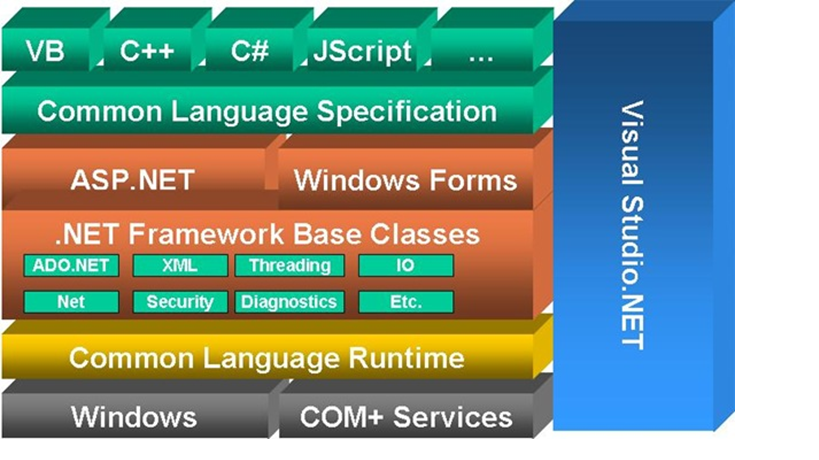
\includegraphics[scale=0.6]{image/kienTrucDotNet.png}
    \end{center}
    \caption{Kiến trúc .Net Framework}
    \label{refhinh2_1}
    \end{figure}
\end{center}
\subsection{Mono}
Mono là một nền tảng open-source với mục đích chính là tạo những ứng dụng cross-platform trên nền .Net. Chúng ta có thể sử dụng Mono trên các hệ điều hành như Unix, Linux, Mac OS X, Solaris và tất nhiên là Windows. Bất kì ngôn ngữ nào được biên dịch thành mã IL thuần túy đều có thể tương thích với Mono. Ngoài ra, Mono còn cung cấp thư viện hỗ trợ rất nhiều loại ngôn ngữ lập trình khác như Java, PHP, Python, Object Pascal, Cobra… Mono framework được sử dụng để lập trình ứng dụng mobile và game 2D, 3D. Các thành phần chính của Mono Framework:
\begin{itemize}
\item Mono runtime: cung cấp trình biên dịch Just-in-Time (JIT), Ahead-of-Time (AOT), thực thi, quản lý các tiến trình và giao tiếp với hệ thống.
\item C\# Compiler: bao gồm các công cụ
\begin{itemize}
\item mcs: (phiên bản 1.1) hỗ trợ C\# 1.0 và C\# 3.0 ngoại trừ các tính năng về generic.
\item gmcs: (phiên bản 2.0) hỗ trợ đầy đủ C\# 3.0.
\item smcs: (phiên bản 2.1) hỗ trợ thêm Silverlight/Moonlight.
\item dmcs: (phiên bản 4.0) hỗ trợ C\# 4.0.
\end{itemize}
\item Base Class Library: thư viện nền tảng để phát triển ứng dụng, tương thích với .Net framework.
\item Mono Class Library: Cung cấp các thư viện lập trình như Gtk+, Zip files, LDAP, OpenGL, Cairo, POSIX,… \cite{4}
\end{itemize}
\subsection{.NET Core}
.NET Core là một framework mã nguồn mở mới và framework đa nền tảng (cross-platform) cho việc xây dựng những ứng dụng hiện tại dựa trên kết nối đám mây, giống như web apps, IoT và backend cho mobile. Ứng dụng ASP.NET Core có thể chạy trên .NET Core hoặc trên phiên bản đầy đủ của .NET Framework. Nó được thiết kế để cung cấp và tối ưu hệ thống đang và đã phát triển cho những ứng dụng được triển khai trên đám mây (cloud) hoặc chạy on-promise. Nó bao gồm các thành phần theo hướng module nhằm tối thiểu tài nguyên và chi phí phát triển. Chúng ta có thể phát triển và chạy những ứng dụng ASP.NET Core đa nền tảng trên Windows, Mac và Linux. Đồng thời nó đã trở thành một mã nguồn mở. Đây là một thay đổi rất lớn và theo em là quan trọng nhất của ASP.NET Core. Điều mà trước đây khó có một lập trình viên nào có thể nghĩ đến. Có lẽ đó cũng là một xu thế mà các ngôn ngữ lập trình hiện nay đang hướng tới.
\par
Bản phát hành đầu tiên của ASP.NET đã xuất hiện cách đây 15 năm trước, nó là một phần của .NET Framework. Từ đó, hàng triệu lập trình viên đã sử dụng nó để xây dựng những ứng dụng web tuyệt vời, và trên những năm đó Microsoft đã phát triển thêm nhiều tính năng mới.ASP.NET Core có một số thay đổi kiến trúc lớn, đó là kết quả của việc học hỏi rất nhiều từ các framework module hóa khác. ASP.NET Core không còn dựa trên System.Web.dll nữa. Nó được dựa trên một tập hợp các gói, các module hay cũng được gọi là các Nuget packages. Điều này cho phép chúng ta tối ưu ứng dụng để chỉ bao gồm những packages nào cần thiết. Lợi ích của nó là giúp cho ứng dụng nhỏ hơn, bảo mật chặt chẽ hơn, giảm sự phức tạp, tối ưu hiệu suất hoạt động và giảm chi phí, thời gian cho việc phát triển. Với ASP.NET Core chúng ta đạt được những nền tảng cải tiến dưới đây:
\begin{itemize}
\item Hợp nhất việc xây dựng web UI và web APIs.
\item Tích hợp những client-side frameworks hiện đại và những luồng phát triển.
\item Hệ thống cấu hình dựa trên môi trường đám mây thật sự.
\item Dependency injection được xây dựng sẵn.
\item HTTP request được tối ưu nhẹ hơn.
\item Có thể host trên IIS hoặc self-host trong process của riêng project hiện tại.
\item Được xây dựng trên .NET Core, hỗ trợ thực sự app versioning.
\item Chuyển các thực thể, thành phần, module như những NuGet packages
\item Những công cụ mới để đơn giản hóa quá trình phát triển web hiện đại
\item Xây dựng và chạy đa nền tảng(Windows, Mac và Linux)
\item Mã nguồn mở và tập trung vào cộng đồng
\end{itemize}
\subsection{Vòng đời yêu cầu trong ASP.NET}
Trong ASP.NET có 2 loại vòng đời:
\begin{itemize}
	\item Vòng đời của ứng dụng là quá trình ứng dụng thực sự bắt đầu chạy IIS cho đến khi nó dừng lại. Vòng đời ứng dụng có thể chia thành các giai đoạn sau:
	\begin{itemize}
		\item Người dùng gửi yêu cầu truy cập vào dữ liệu của ứng dụng và trình duyệt sẽ gửi yêu cầu này đến Web Server
		\item Các sự kiện sau đây sẽ được khởi tạo:
		\begin{itemize}
			\item Một đối tượng của lớp ApplicationManager được tạo.
			\item Một đối tượng lớp HostingEvironment được tạo để cung cấp thông tin về nguồn dữ liệu.
			\item Các thành phần đầu của ứng dụng sẽ được biên dịch.
		\end{itemize}
		\item Các đối tượng HttpContext, HttpRequest và HttpResponse được khởi tạo và cài đặt.
		\item Một thể hiện của đối tượng HttpApplication được tạo và gắn cho yêu cầu.
		\item Các yêu cầu được xử lý bởi lớp HttpApplication, các sự kiện khác nhau được kích hoạt bởi lớp này để xử lý các yêu cầu.
	\end{itemize}
	\item Vòng đời của yêu cầu gửi lên server.
\end{itemize}
\begin{center}
    \begin{figure}[h]
    \begin{center}
     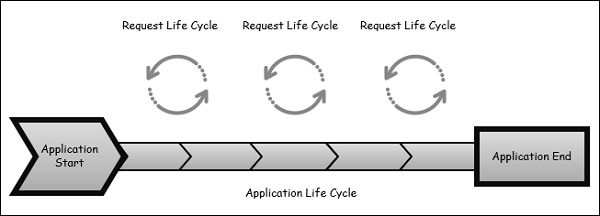
\includegraphics[scale=1.0]{image/vongdoiMVC.png}
    \end{center}
    \caption{Tổng quan vòng đời trong ASP.NET nói chung}
    \label{refhinh2_4}
    \end{figure}
\end{center}
\par
Hình \ref{refhinh2_4} là một vòng đời của một ứng dụng trong nền tảng .NET. Ta có thể thấy trong một vòng đời ứng dụng có rất nhiều các yêu cầu gửi lên từ các user cho server xử lý, mỗi một vòng đời của một yêu cầu gửi lên cho server xử lý sẽ chứa rất nhiều sự kiện mà người dùng thao tác và mong muốn server trả kết quả ra ngoài màn hình. Kết thúc một vòng đời một của yêu cầu hệ thống sẽ tự động đóng kết nối và dọn những thực thể mà yêu cầu đã sử dụng.
\begin{center}
    \begin{figure}[h]
    \begin{center}
     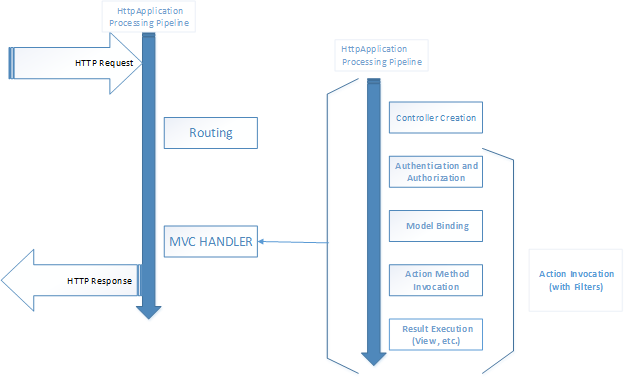
\includegraphics[scale=1.0]{image/vongdoiMVCchitiet.png}
    \end{center}
    \caption{Vòng đời trong ASP.NET MVC}
    \label{refhinh2_5}
    \end{figure}
\end{center}
\par
Hình \ref{refhinh2_5} là hình mô tả chi tiết vòng đời trong ASP.NET MVC ở mức 2 level. Khi có 1 yêu cầu gửi lên ứng dụng sẽ có một chuỗi sự kiện được xử lý ở server, nó sẽ được định tuyến qua 1 đường ống xử lý trong lớp HttpApplication để đến được đúng Controller và Action của nó, khi vào Controller sự kiện đấy phải được kiểm tra quyền đăng nhập và quyền ứng dụng nếu ứng dụng có cài đặt 2 quyền trên, sau đó là bước truyền các tham số vào cho Action xử lý nếu qua được bước kiểm tra quyền cuối cùng Action sẽ trả về 1 kết quả cho Controller gửi ra View và trả về 1 kết quả được hiển thị cho người dùng thông qua View.
\begin{center}
    \begin{figure}[h]
    \begin{center}
     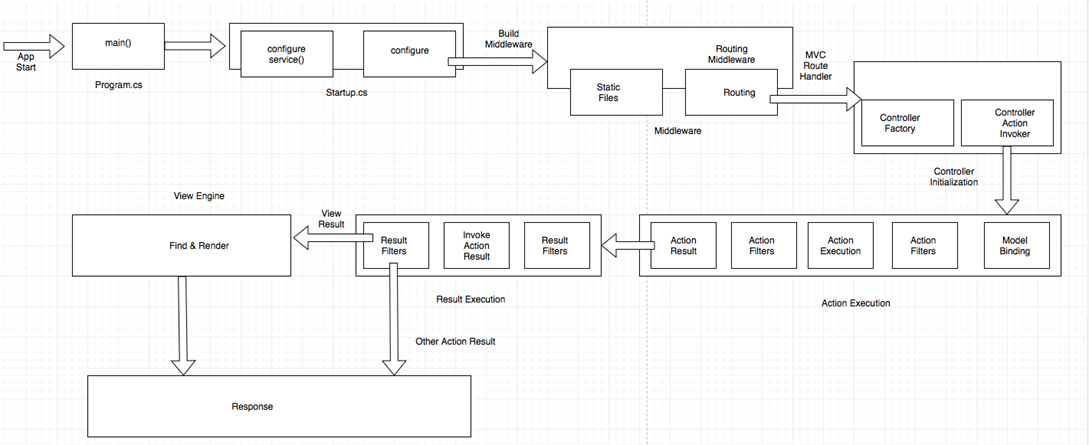
\includegraphics[scale=0.6]{image/vongdoiCore.png}
    \end{center}
    \caption{Vòng đời trong ASP.NET Core}
    \label{refhinh2_6}
    \end{figure}
\end{center}
\par
Hình \ref{refhinh2_6} mô tả chi tiết vòng đời trong ASP.NET Core. Khi có một yêu cầu gửi đến server nó cũng sẽ được định tuyến qua 1 URL nhất định, vì ASP.NET Core được thiết kế theo dạng module hoá nên các module được khởi tạo và sử dụng được khai báo trong file StartUp.cs trong đó phương thức ConfigureServices() để khai báo những module được sử dụng trong hệ thống, còn phương thức Configure() được sử dụng để sử dụng các module đã khai báo. Sau đấy qua tầng Middleware là tầng ở giữa để xử lý định tuyến URL và những file tĩnh trong hệ thống như: file css, js,... Ở tầng Middleware này, lập trình viên có thể lập trình cho hệ thống gửi kèm một số thứ lên cùng với yêu cầu người dùng như là gửi kèm 1 header để xác thực người dùng chẳng hạn. Sau khi định tuyến được yêu cầu thì server xử lý các tham số của yêu cầu vào trong Controller, ở Controller các thể hiện sẽ được tiêm vào hàm tạo của Controller theo cơ chế Dependency Injection. Sau khi xử lý thành công ở Controller thì hệ thống sẽ trả lại kết quả đến hiển thị trên View cho người dùng. 
\section{CSHTML}
CSHTML là 1 view engine dùng để xử lý và tạo HTML, nó là 1 view để nhận các dữ liệu mà controller gửi đến, CSHTML cho phép viết mã nguồn C\# để xử lý dữ liệu trên view dễ dàng hơn. CSHTML sử dụng Raroz để viết mã. Cơ chế Razor giảm thiểu số lượng ký tự và phím nhấn cần để tạo một tập tin View, do đó lập trình viên có thể làm việc nhanh và trôi chảy hơn. Khi chạy trên môi trường web thì file CSHTML sẽ tự động trở thành mã HTML để hiển thị lên các trình duyệt website
\section{Bootstrap}
Bootstrap là 1 framework HTML, CSS, và JavaScript cho phép người dùng dễ dàng thiết kế website theo 1 chuẩn nhất định, tạo các website thân thiện với các thiết bị cầm tay như mobile, ipad, tablet,...
\par
Bootstrap bao gồm những cái cơ bản có sẵn như: typography, forms, buttons, tables, navigation, modals, image carousels và nhiều thứ khác. Trong bootstrap có thêm nhiều Component, Javascript hỗ trợ cho việc thiết kế reponsive của chúng ta dễ dàng, thuận tiện và nhanh chóng hơn. Nên dùng bootstrap để viết giao diện front-end vì:
\begin{itemize}
\item Bootstrap là một trong những framework được sử dụng nhiều nhất trên thế giới để xây dựng nên một website. Bootstrap đã xây dựng nên 1 chuẩn riêng và rất được người dùng ưa chuộng. Chính vì thế, chúng ta hay nghe tới một cụm từ rất thông dụng "Thiết kế theo chuẩn Bootstrap".
\item Rất dễ để sử dụng: Nó đơn giản vì nó được base trên HTML, CSS và Javascript chỉ cần có kiến thức cơ bản về ba ngôn ngữ nêu trên là có thể sử dụng bootstrap tốt.
\item Responsive: Bootstrap xây dựng sẵn reponsive css trên các thiết bị Iphones, tablets, và desktops. Tính năng này khiến cho người dùng tiết kiệm được rất nhiều thời gian trong việc tạo ra một website thân thiện với các thiết bị điện tử, thiết bị cầm tay.
\item Tương thích với trình duyệt: Nó tương thích với tất cả các trình duyệt (Chrome, Firefox, Internet Explorer, Safari, and Opera). Tuy nhiên, với IE browser, Bootstrap chỉ hỗ trợ từ IE9 trở lên. Điều này vô cùng dễ hiểu vì IE8 không support HTML5 và CSS3.
\end{itemize}

\section{Jquery Ajax}
\subsection{Jquery}
jQuery là một Framework được xây dựng dựa trên các tính năng của JavaScript. Vì thế trong khi phát triển các ứng dụng sử dụng jQuery, chúng ta có thể sử dụng tất cả các hàm và các tính năng khác được bổ trợ trong JavaScript. jQuery làm đơn giản hóa việc truyền tải HTML, xử lý sự kiện, tạo hiệu ứng động và tương tác Ajax. Với jQuery, khái niệm Rapid Web Development đã không còn quá xa lạ. jQuery là một bộ công cụ tiện ích JavaScript làm đơn giản hóa các tác vụ đa dạng với việc viết ít code hơn. Dưới đây liệt kê một số tính năng tối quan trọng được hỗ trợ bởi jQuery:
\begin{itemize}
\item Thao tác DOM: jQuery giúp dễ dàng lựa chọn các phần tử DOM để traverse (duyệt) một cách dễ dàng như sử dụng CSS, và chỉnh sửa nội dung của chúng bởi sử dụng phương tiện Selector mã nguồn mở, mà được gọi là Sizzle.
\item Xử lý sự kiện: jQuery giúp tương tác với người dùng tốt hơn bằng việc xử lý các sự kiện đa dạng mà không làm cho HTML code rối tung lên với các Event Handler.
\item Hỗ trợ AJAX: jQuery giúp chúng ta rất nhiều để phát triển một site giàu tính năng và phản hồi tốt bởi sử dụng công nghệ AJAX.
\item Hiệu ứng: jQuery đi kèm với rất nhiều các hiệu ứng đa dạng và đẹp mắt mà chúng ta có thể sử dụng trong các Website của mình.
\item Gọn nhẹ: jQuery là thư viện gọn nhẹ - nó chỉ có kích cỡ khoảng 19KB (gzipped).
\item Được hỗ trợ hầu hết bởi các trình duyệt hiện đại: jQuery được hỗ trợ hầu hết bởi các trình duyệt hiện đại, và làm việc tốt trên IE 6.0+, FF 2.0+, Safari 3.0+, Chrome và Opera 9.0+
\end{itemize}


    \begin{longtable}{m{0.1\linewidth}  m{0.3\linewidth}  m{0.5\linewidth}}
    \caption{Các hàm có sẵn trong Jquery \cite{3}} \\ \hline
     	\textbf{STT} & \textbf{Tên hàm} & \textbf{Mô tả hàm} \\ \hline
     	1&charAt()&Trả về ký tự tại chỉ mục (index) đã cho. \\
		\hline
     	2&concat()&Kết nối hai chuỗi văn bản và trả về một chuỗi mới.\\
		\hline
     	3&forEach()&Gọi một hàm cho mỗi phần tử của một mảng.\\
     	\hline
     	4&indexOf()&Trả về chỉ mục về sự xuất hiện đầu tiên bên trong việc gọi đối tượng String với giá trị đã cho, hoặc -1 nếu không tìm thấy.\\
     	\hline
     	5&length()&Trả về độ dài của chuỗi.\\
     	\hline
     	6&pop()&Gỡ bỏ phần tử cuối của một mảng và trả về phần tử đó.\\
     	\hline
		7&push()&Thêm một hoặc nhiều phần tử tới phần cuối của một mảng và trả về độ dài mới của mảng đó.\\
		\hline
		8&reverse()&Đảo ngược thứ tự các phần tử trong một mảng – phần tử đầu tiên thành cuối cùng và cuối cùng thành đầu tiên.\\
		\hline
		9&sort()&Sắp xếp phân loại các phần tử của một mảng.\\
		\hline
		10&substr()&Trả về các ký tự trong một mảng bắt đầu từ vị trí đã cho từ số các ký tự đã xác định.\\
		\hline
		11&toLowerCase()&Trả về giá trị chuỗi đang gọi được biến đổi thành kiểu chữ thường.\\
		\hline
		12&toString()&Trả về sự biểu diễn chuỗi của giá trị số.\\
		\hline
		13&toUpperCase()&Trả về giá trị chuỗi đang gọi được biến đổi thành chữ hoa. \\ \hline
	\label{bang2_1}
    \end{longtable}
\subsection{Ajax}
Ajax là một bộ công cụ cho phép load dữ liệu từ server mà không yêu cầu tải lại trang. Nó sử dụng chức năng sẵn có XMLHttpRequest(XHR) của trình duyệt để thực hiện một yêu cầu đến server và xử lý dữ liệu server trả về.
\par
\textit{Ví dụ} : khi một người dùng viết một nhận xét trên bài viết đăng trên trang Facebook. Sau khi người dùng gửi nhận xét thành công trang Facebook mà người đó đang truy cập cần phải được cập nhật để hiển thị nhận xét vừa mới được tạo ra này. Nếu load lại toàn bộ trang mà người dùng đang truy cập thì sẽ không hiệu quả do tất cả những gì chúng ta muốn là hiển thị nhận xét mới được tạo ra, Ajax được tạo ra để giải quyết vấn đề này, thay vì tải lại toàn bộ trang trình duyệt sẽ chỉ tải những phần được thay đổi để tiết kiệm thời gian chờ đợi một lượng thông tin lớn về từ server.\par
Một số ứng dụng sử dụng Ajax như : Gmail , Google Maps , Youtube , Facebook,...\par
Jquery cung cấp một số phương thức để thực hiện các chức năng ajax. Chúng ta có thể yêu cầu các text, HTML, XML và JSON từ server sử dụng cả giao thức HTTP GET và HTTP POST, chúng ta cũng có thể lấy dữ liệu từ bên ngoài trực tiếp vào trong phần tử được chọn.
\begin{itemize}
\item  Phương thức jquery load()
\begin{lstlisting}
	$(selector).load(URL,data,callback);
\end{lstlisting}
\begin{itemize}
\item Phương thức load() lấy dữ liệu từ server và trả dữ liệu cho phần tử được chọn.
\item URL: mà chúng ta muốn lấy dữ liệu.
\item Data: cặp key/value gửi đi cùng với yêu cầu.
\item Callback: tên của hàm sẽ được thực thi sau khi phương thức load hoàn thành.
\end{itemize}
\item Phương thức Post trong JQuery Ajax
\begin{lstlisting}
	$(selector).post(URL,data,function(data,status,xhr),dataType)	
\end{lstlisting}
\begin{itemize}
	\item Có tác dụng lấy dữ liệu từ server bằng phương thức HTTP POST REQUEST
	\item URL: required , đường dẫn đến file cần lấy thông tin.
	\item Data: không bắt buộc ,là một đối tượng object gồm các key và value sẽ gửi lên server.
	\item function(data, status , xhr): là function sẽ xử lý khi thực hiện thành công với các parameters:
	\begin{itemize}
		\item  Data : bao gồm các dữ liệu trả về từ request.
		\item  Status : gồm trạng thái request (“success” , “notmodified” , “error” , “timeout” , or “parsererror”).
		\item  Xhr : gồm các đối tượng XMLHttpRequest.
	\end{itemize}
	\item  dataType: là dạng dữ liệu trả về. (text, json, script, xml,html,jsonp )
\end{itemize}
\item Phương thức Get trong Jquery Ajax
\begin{lstlisting}
	$(selector).post(URL,data,function(data,status,xhr),dataType)
\end{lstlisting}	
\begin{itemize}
	\item Có tác dụng lấy dữ liệu từ server bằng phương thức HTTP POST REQUEST.
	\item Các thành phần tương tự như phương thức Post.
\end{itemize}
\end{itemize}
\section{Phần mềm hỗ trợ và phát triển website}
\subsection{Visual Studio}
Visual Studio là (IDE – Integrated Development Environment) một bộ công cụ phát triển phần mềm do Microsoft phát triển. Visual Studio cũng là một phần mềm được sử dụng bởi các lập trình viên để xây dựng nên các sản phẩm phần mềm. Nó được sử dụng để phát triển chương trình máy tính cho Microsoft Windows, cũng như các trang web, các ứng dụng web và các dịch vụ web. Visual Studio sử dụng nền tảng phát triển phần mềm của Microsoft như Windows API, Windows Forms, Windows Presentation Foundation, Windows Store và Microsoft Silverlight. Nó có thể sản xuất cả hai ngôn ngữ máy và mã số quản lý.
\par
Visual Studio bao gồm một trình soạn thảo mã hỗ trợ IntelliSense cũng như cải tiến mã nguồn. Trình gỡ lỗi tích hợp hoạt động cả về trình gỡ lỗi mức độ mã nguồn và gỡ lỗi mức độ máy. Công cụ tích hợp khác bao gồm một mẫu thiết kế các hình thức xây dựng giao diện ứng dụng, thiết kế web, thiết kế lớp và thiết kế giản đồ cơ sở dữ liệu. Nó chấp nhận các plug-in nâng cao các chức năng ở hầu hết các cấp bao gồm thêm hỗ trợ cho các hệ thống quản lý phiên bản (như Subversion) và bổ sung thêm bộ công cụ mới như biên tập và thiết kế trực quan cho các miền ngôn ngữ cụ thể hoặc bộ công cụ dành cho các khía cạnh khác trong quy trình phát triển phần mềm.
\par
Em chọn Visual Studio bởi nó có những điểm mạnh sau đây:
\begin{itemize}
	\item Hỗ trợ lập trình trên nhiều ngôn ngữ như C/C++, C\#, F\#, Visual Basic, HTML, CSS, JavaScript. Phiên bản Visual Studio 2015 có hỗ trợ ngôn ngữ Python.
	\item Visual Studio là một công cụ hỗ trợ việc Debug một cách mạnh mẽ, dễ dàng nhất (Break Point, xem giá trị của biến trong quá trình chạy, hỗ trợ debug từng câu lệnh).
	\item Giao diện Visual Studio rất dễ sử dụng đối với người mới bắt đầu.
	\item Visual Studio hỗ trợ phát triển ứng dụng desktop MFC, Windows Form, Universal App, ứng dụng mobileWindows Phone 8/8.1, Windows 10, Android (Xamarin), iOS và phát triển  website Web Form, ASP.NET MVC và phát triển Microsoft Office.
	\item Visual Studio hỗ trợ kéo thả để xây dựng ứng dụng một cách chuyên nghiệp, giúp các lập trình viên mới bắt đầu có thể tiếp cận nhanh hơn.
	\item Visual Studio cho phép chúng ta tích hợp những extension từ bên ngoài như Resharper (hỗ trợ quản lý và viết mã nhanh cho các ngôn ngữ thuộc .Net), hay việc cài đặt thư viện nhanh chóng thông qua Nuget
	\item Visual Studio được sử dụng đông đảo bởi lập trình viên trên toàn thế giới.
\end{itemize}
\subsection{Visual Studio Code}
Visual Studio Code là sản phẩm của Microsoft, ra mắt vào tháng 4 năm 2015 ở hội nghị Build. Đặc điểm nổi bật là đơn giản, gọn nhẹ, dễ dàng cài đặt. Visual Studio Code có thể cài đặt được trên cả Windows, Linux và Mac OS và hỗ trợ nhiều ngôn ngữ. Điểm mạnh của Visual Studio Code:
\begin{itemize}
	\item VS Code còn hỗ trợ tất cả các ngôn ngữ lập trình trên nhiều nền tảng khác nhau với bộ thư viện Extension phong phú. VS Code cũng là một công cụ phát triển web rất tốt.
	\item VS Code chỉ tập trung quản trị code trên đơn vị file (như một công cụ text-editor), không như Visual Studio thiên về project và solution. Đặc điểm này giống với Sublime hay Atom. Cũng dễ hiểu khi VS Code cũng được xây dựng trên nền Electron như Sublime.
	\item VS Code với trình gợi ý và tính năng auto-completion tích hợp trí tuệ nhân tạo sẽ đem đến cho chúng ta một trải nghiệm mới hơn và tiện lợi hơn.
	\item VS Code cũng tích hợp Git cũng như bộ command của nó giúp developer có thể nhanh chóng tải và cài đặt các project từ Git repo.
	\item Đặc biệt VS Code là miễn phí nếu không muốn nói là mã nguồn mở.
\end{itemize}
\subsection{Microsoft Sql Server Management Studio}
\subsubsection{Khái niệm về SQL Server}
SQL Server chính là một hệ quản trị dữ liệu sử dụng câu lệnh SQL để trao đổi dữ liệu giữa máy cài SQL Server và máy Client. Một Relational Database Management System – RDBMS gồm có: databases, datase engine và các chương trình ứng dụng dùng để quản lý các bộ phận trong RDBMS và những dữ liệu khác.
\subsubsection{Lịch sử ra đời và các phiên bản của SQL Server}
Năm 1989, phiên bản đầu tiên của SQL Server 1.0 ra đời được dùng cho các hệ điều hành 16 bit và được phát triển cho tới ngày nay.
\par
Cho tới khi SQL Server ra phiên bản 6.5 thì được thị trường chấp nhận rộng rãi. Một đột phá cải tiến cho SQL Server 7.0 khi được Microsoft viết lại một engine hoàn toàn mới. Đến khi SQL Server từ phiên bản 7.0 cải tiến lên 8.0 chủ yếu phát triển về tính năng thiết kế web.
\par
Cho đến ngày nay thì phiên bản mới nhất đó là SQL Server 2017 hỗ trợ bộ vi xử lý 64 bit ra đời vào ngày 1 tháng 6 năm 2017. Cho đến nay SQL Server có 5 phiên bản:
\begin{itemize}
\item 	Enterprise: là một ấn bản chứa tất cả các đặc điểm nổi bật của SQL Server như: các công cụ cho tạo và quản lý phân cụm SQL Server, nhân bộ máy cơ sở dữ liệu và một số dịch vụ đi kèm. Nó có thể đánh địa chỉ 12 terabytes và quản lý cơ sở dữ liệu lên tới 524 petabytes.
\item 	Standard: Ấn bản này có thể chạy tốt trên hệ thống lên tới 4 CPU và 2 GB RAM rất thích hợp cho các dịch vụ thiết kế web vừa và nhỏ.
\item	Developer: Ấn bản này giới hạn số lượng người kết nối với server nhưng có đầy đủ các tính năng của Enterprise Edition. Đây là phiên bản được sử dụng cho kiểm tra và phát triển ứng dụng phù hợp cho các cá nhân trong lĩnh vực web như: freelancer Việt Nam.
\item	Workgroup: ấn bản SQL Server này có các chức năng lõi cơ sở dữ liệu nhưng không đi kèm các dịch vụ. Ở phiên bản 2012 không có ấn bản này.
\item	Express: Ấn bản này dễ dàng sử dụng và quản trị cơ sở dữ liệu đơn giản.
\end{itemize}
\subsubsection{Các thành phần cơ bản trong SQL Server}
Các thành cơ bản trong SQL Server gồm có: Reporting Services, Database Engine, Integration Services, Notification Services, Full Text Search Service, … Tất cả kết hợp với nhau tạo thành một giải pháp hoàn chỉnh giúp cho việc phân tích và lưu trữ dữ liệu trở nên dễ dàng hơn.
\begin{itemize}
\item	Database Engine: Đây là một engine có khả năng chứa dữ liệu ở các quy mô dưới dạng support và table. Ngoài ra, nó còn có khả năng tự điều chỉnh ví dụ: trả lại tài nguyên cho hệ điều hành khi một user log off và sử dụng thêm các tài nguyên của máy khi cần.
\item	Integration Services: là tập hợp các đối tượng lập trình và các công cụ đồ họa cho việc sao chép, di chuyển và chuyển đổi dữ liệu.  Khi bạn làm việc trong một công ty lớn thì dữ liệu được lưu trữ ở nhiều nơi khác nhau như được chứa trong: Oracle, SQL Server, DB2, Microsoft Access, … và bạn chắc chắn sẽ có nhu cầu di chuyển dữ liệu giữa các server này. Ngoài ra, bạn còn muốn định dạng dữ liệu trước khi lưu vào database. Chắc chắn Integration Services sẽ giúp bạn giải quyết được công việc này dễ dàng.
\item	Analysis Services: Đây là một dịch vụ phân tích dữ liệu rất hay của Microsoft. Dữ liệu khi được lưu trữ vào trong database mà bạn không thể lấy được những thông tin bổ ích thì coi như không có ý nghĩa gì. Chính vì thế, công cụ này ra đời giúp bạn trong việc phân tích dữ liệu một cách hiệu quả và dễ dàng bằng cách dùng kỹ thuật khai thác dữ liệu – datamining và khái niệm hình khối nhiều chiều – multi dimendion cubes.
\item	Notification Services: Dịch vụ thông báo này là nền tảng cho sự phát triển và triển khai các ứng dụng soạn và gửi thông báo. Ngoài ra, dịch vụ này còn có chức năng gửi thông báo theo dịch thời đến hàng ngàn người đăng ký sử dụng trên nhiều loại thiết bị khác nhau.
\item	Reporting  Services: là một công cụ tạo, quản lý và triển khai báo cáo bao gồm: server và client. Ngoài ra, nó còn là nền tảng cho việc phát triển và xây dựng các ứng dụng báo cáo.
\item	Full Text Search Service: là một thành phần đặc biệt trong việc truy vấn và đánh chỉ mục dữ liệu văn bản không cấu trúc được lưu trữ trong các cơ sở dữ liệu SQL Server.
\item	Service Broker: là một môi trường lập trình cho việc tạo ra các ứng dụng trong việc nhảy qua các Instance.
\end{itemize}
\subsubsection{Tại sao sử dụng SQL Server trong thiết kế website}
SQL Server không phải là một hệ quản trị cơ sở dữ liệu độc lập mà nó chỉ là một thành phần với vai trò ngôn ngữ là công cụ giao tiếp giữa hệ cơ sở dữ liệu và người dùng. Chính vì thế nó được sử dụng trong các dịch vụ thiết kế web đẹp với chức năng giao tiếp với người dùng có các vai trò sau:
\begin{itemize}
\item	SQL là một ngôn ngữ đòi hỏi có tính tương tác cao: Người dùng có thể dễ dàng trao đổi với các tiện ích thông qua các câu lệnh của SQL đến cơ sở dữ liệu và nhận kết quả từ cơ sở dữ liệu.
\item	SQL là một ngôn ngữ lập trình cơ sở dữ liệu: Các lập trình viên có thể xây dựng các chương trình ứng dụng giao tiếp với cơ sở dữ liệu bằng cách nhúng các câu lệnh SQL vào trong ngôn ngữ lập trình.
\item	SQL là một ngôn ngữ lập trình quản trị cơ sở dữ liệu: Người quản trị cơ sở dữ liệu có thể quản lý, định nghĩa và điều khiển truy cập cơ sở dữ liệu thông qua SQL.
\item	SQL là một ngôn ngữ lập trình cho các hệ thống chủ khách: SQL được sử dụng như là một công cụ giao tiếp với các trình ứng dụng trong hệ thống cơ sở dữ liệu khách chủ.
\item	SQL là ngôn ngữ truy cập dữ liệu trên Internet: SQL được sử dụng với vai trò tương tác với dữ liệu trong hầu hết các máy chủ web và máy chủ Internet.
\item	SQL là ngôn ngữ cơ sở dữ liệu phân tán: Với vai trò giao tiếp với các hệ thống trên mạng, gửi và nhận các yêu cầu truy xuất dữ liệu với nhau.

\end{itemize}

\section{Kết luận}
Từ những lý thuyết về các ngôn ngữ lập trình cũng như các Framework mà em đã tìm hiểu, em sẽ vận dụng chúng để thiết kế và triển khai website được trình bày ở các chương \ref{chapter3}.

 






%\chapter{KIẾN TRÚC HỆ THỐNG}
\label{chapter3}
Từ những cơ sở lý thuyết thu thập ở chương 2, chương này em sẽ trình bày những bước giải quyết bài toán mà đề tài đưa ra.
\section{Phân tích yêu cầu}
Từ yêu cầu của đề tài và việc phân tích chi tiết yêu cầu và chức năng của hệ thống cần phải đáp ứng, em đã xác định được yêu cầu chức năng và phi chức năng của hệ thống như sau:
\begin{itemize}
\item	Yêu cầu chức năng:
	\begin{itemize}
	\item	Các nút truyền dữ liệu đến được Gateway,
	\item	Mạng có linh động về số lượng nút,
	\item	Số lượng nút trong mạng từ 3 nút trở lên.
	\end{itemize}
\item Yêu cầu phi chức năng:  
	\begin{itemize}
	\item 	Các nút truyền dữ liệu chính xác, ổn định,
	\item 	Nút tiêu tốn ít năng lượng,
	\item	Thiết bị hoạt động ổn định,
	\item	Hình thức gọn, phù hợp điều kiện làm việc.
	\item	Dữ liệu được đảm bảo an toàn,
	\item	Chi phí hợp lý.
	\end{itemize}
\end{itemize}
\section{Kiến trúc tổng thể hệ thống}
Dựa trên cơ sở kiến trúc đã có sẵn của thiết bị BKRES, hệ thống sẽ được tích hợp thêm module truyền thông LoRa vào các thiết bị của hệ thống. Khi đó hệ thống gồm 4 phân hệ chính. Hình \ref{construction}{} mô tỏ rõ hơn kiến trúc hệ thống.
\begin{itemize}
	\item Phân hệ cảm biến và xử lý dữ liệu: Ở mỗi nút mạng được trang bị các bộ cảm biến ghi đo 4 tham số (hàm lượng Oxy, nhiệt độ, độ pH và nồng độ muối). Dữ liệu cảm biến được gửi đến bộ điều khiển trung tâm (sử dụng vi điều khiển STM32) để xử lý, phân tích, đóng gói và gửi đến module truyền thông LoRa.
	\item Phân hệ truyền thông sử dụng LoRa: hoạt động theo mô hình đơn chặng, có nhiệm vụ gửi dữ liệu từ phân hệ cảm biến tới server trung tâm.
	\item Phân hệ cung cấp dịch vụ: Sau khi nhận dữ liệu từ phân hệ truyền thông, phân hệ này có nhiệm vụ xử lý dữ liệu và cung cấp các dịch vụ cho phân hệ giám sát và người dùng.
	\item Phân hệ giám sát và điều khiển: có nhiệm vụ hiển thị dữ liệu cảm biến một cách trực quan thông qua ứng dụng di động, ứng dụng web. Người dùng có thể cấu hình hệ thống, đặt các mức ngưỡng cảnh báo,… trên ứng dụng.
\end{itemize}
\begin{center}
\begin{figure}
\begin{center}
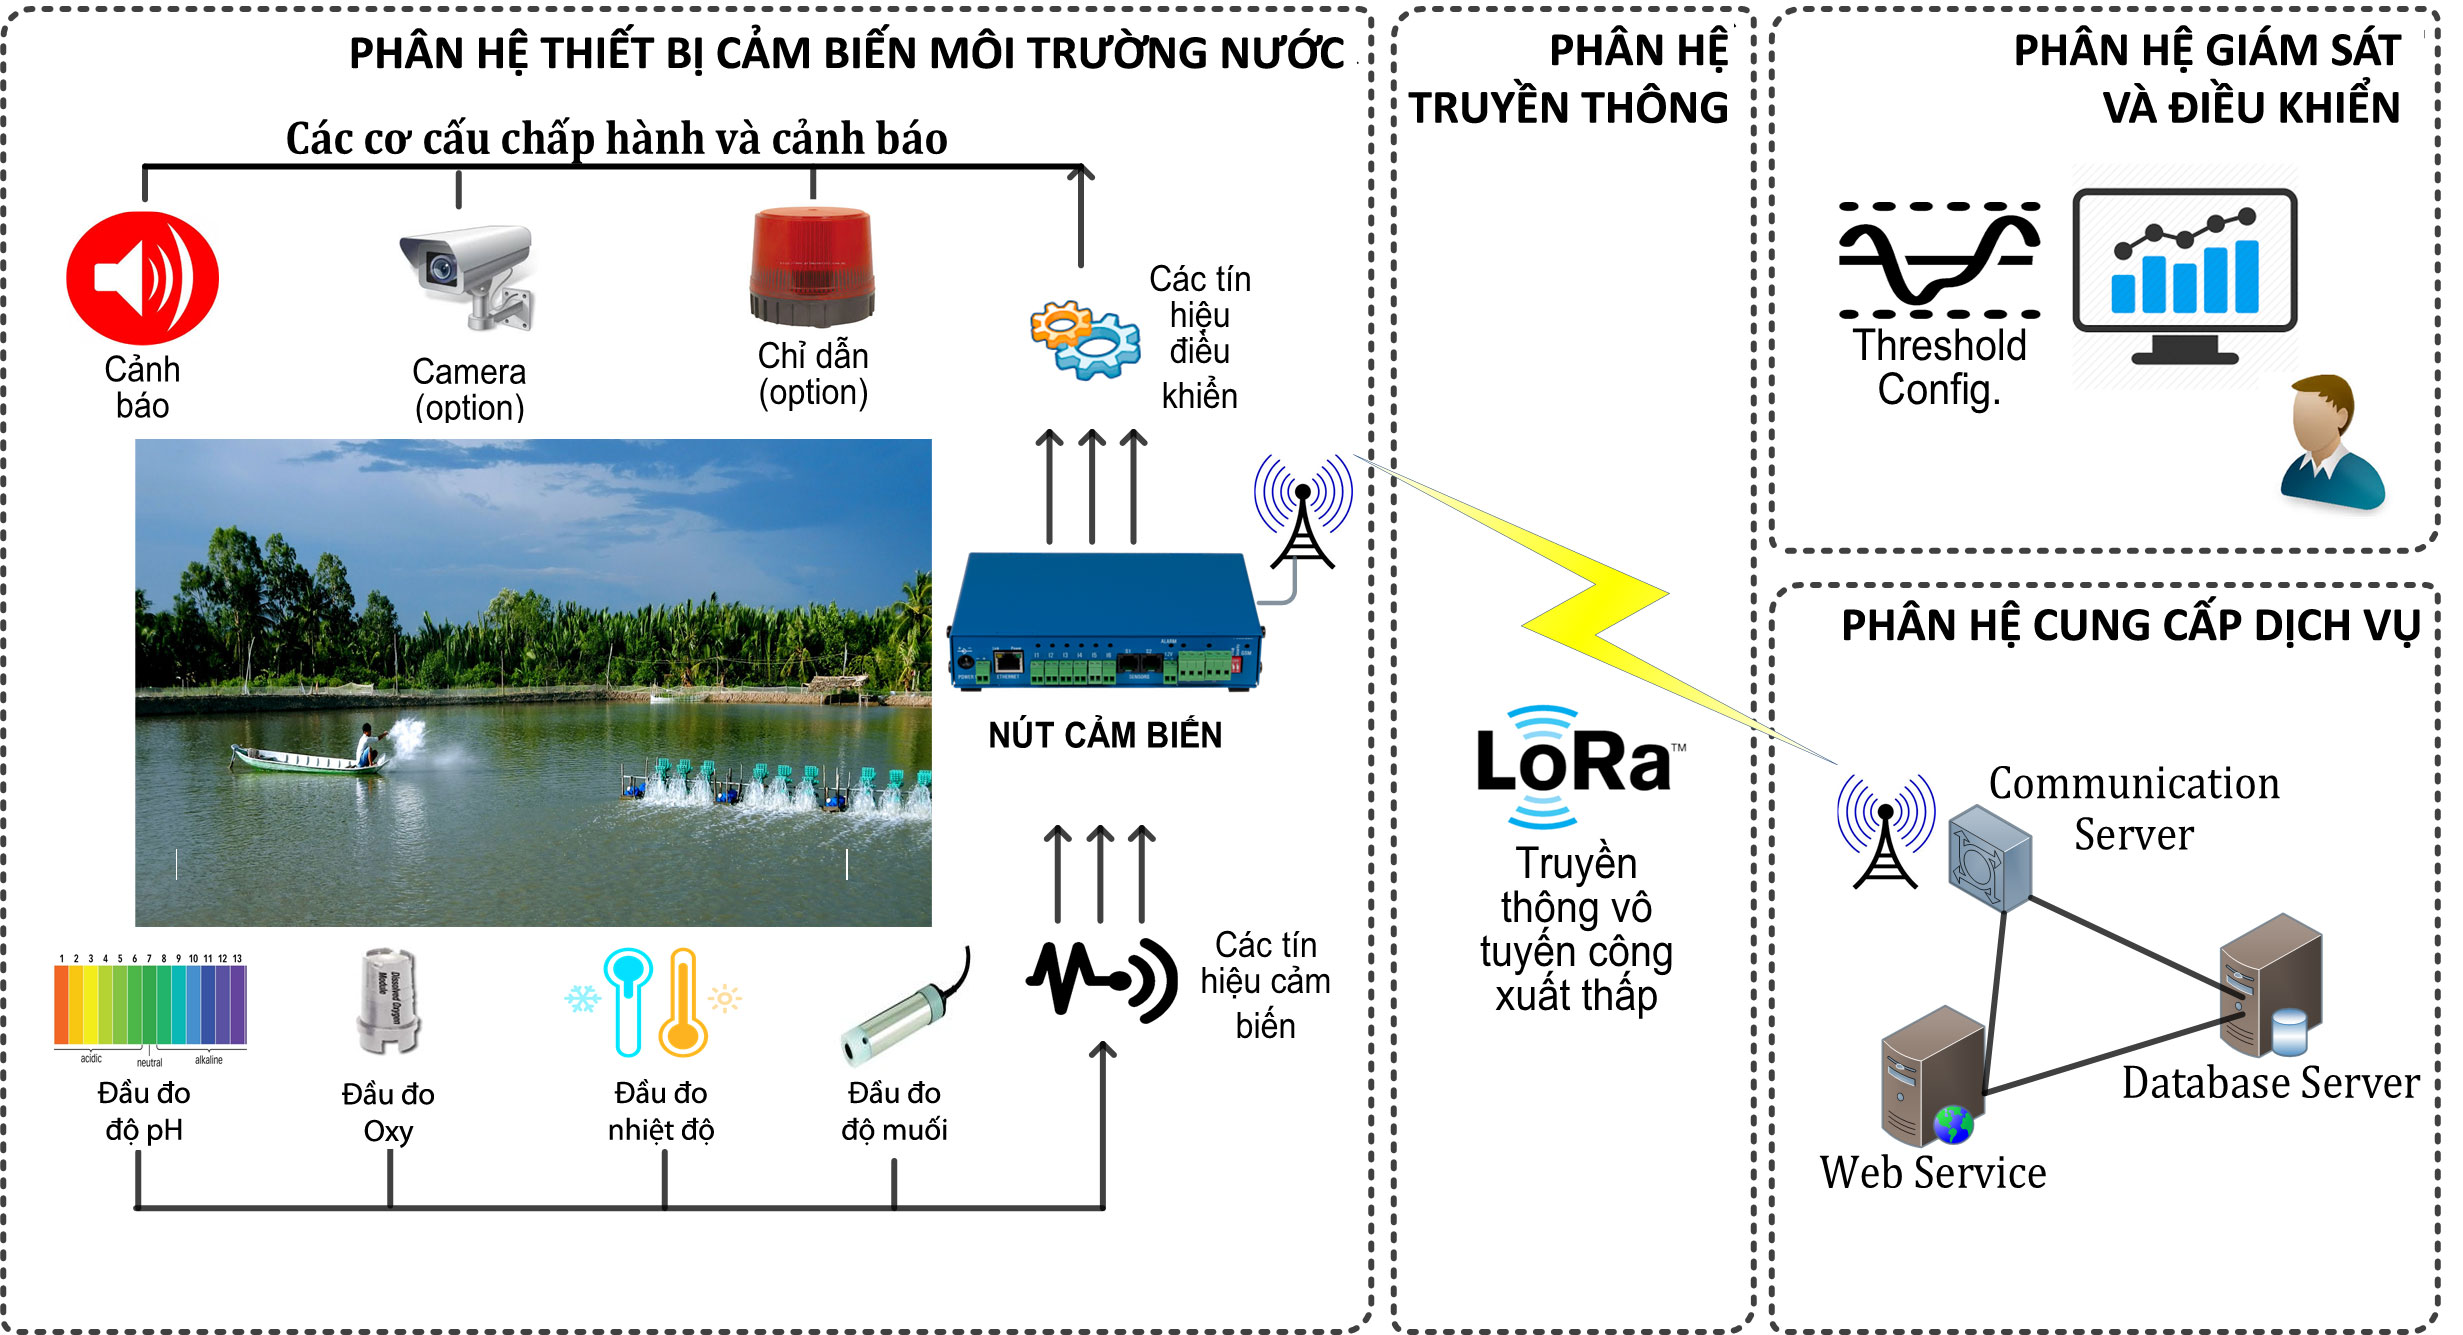
\includegraphics[scale=0.15]{image/kientrucLoRa}
\end{center}
\caption{Kiến trúc hệ thống}
\label{construction}
\end{figure}
\end{center}
\par 
Module LoRa SX1278 được lựa chọn để tích hợp vào thiết bị cảm biến như thể hiện trên hình \ref{moduleSX1278}{}. Nút cảm biến được thiết kế và chế tạo tài phòng nghiên cứu SANSLAB, gồm các thành phần phần cứng chính như: phân hệ cảm biến các tham số môi trường nước, phân hệ truyền thông, phân hệ vi xử lý và điều khiển, phân hệ cấp nguồn và phân hệ hiển thị, cảnh tại chỗ. Phần mềm trên nút cảm biến gồm firmware và drivers điều khiển hoạt động các phân hệ và ngoại vi, thuật toán đa truy nhập cũng được nhúng trong firmware của thiết bị. Một số thuật toán chính được biểu diễn qua các lưu đồ sau đây.
\section{Thiết kế nút mạng cảm biến tích hợp~module SX1278}
%\begin{center}
\begin{figure}[h]
	\begin{center}
		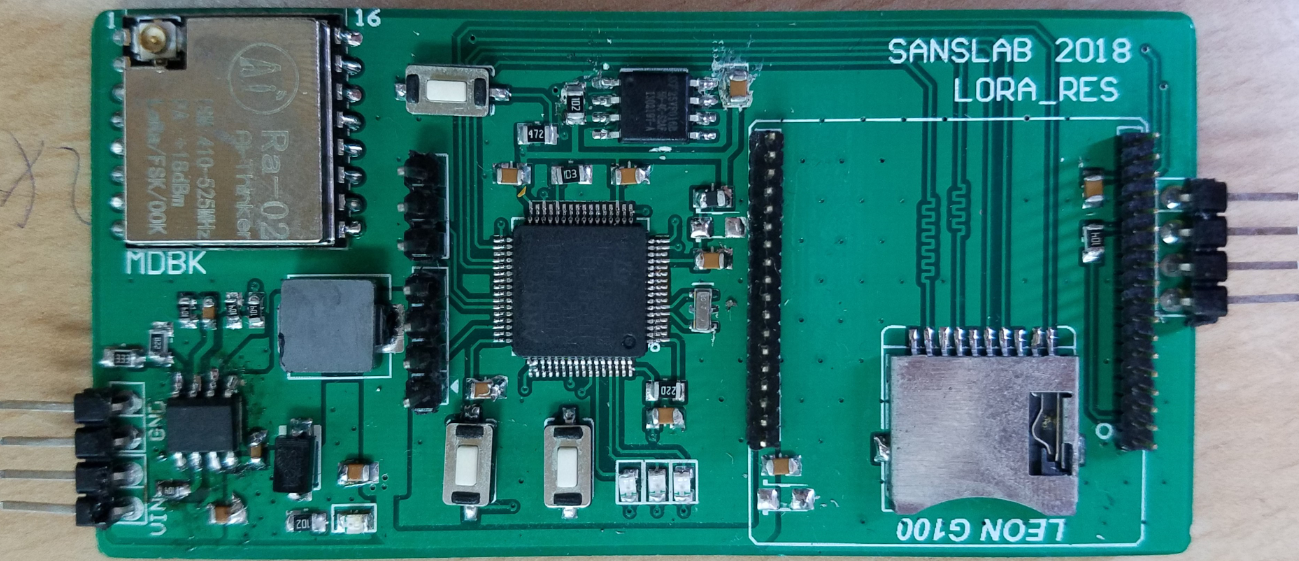
\includegraphics[scale=0.45]{image/hinh3_1}
	\end{center}
	\caption{Nút cảm biến tích hợp chip LoRa SX1278}
	\label{moduleSX1278}
\end{figure}
%\end{center}
\section{Mô hình mạng hình sao}
Thuật toán đa truy nhập đề xuất được phát triển và thử nghiệm trên mô hình gồm 3 nút cảm biến và một Gateway như hình \ref{protocol}{}. Để đánh giá khả năng truyền dữ liệu, độ ổn định, khả năng tùy biến và tự cấu hình của các nút trong mạng, em cấu hình các thông số cơ bản của các nút theo như bảng \ref{bang3_1}{}.
\begin{table}[h]
	\tabcolsep = 2cm
    \centering
    \caption{Bảng thông số cấu hình của các nút trong mạng}
    \begin{tabular}{|c|c|}
     	\hline
     	Thông số & Giá trị  \\
     	\hline
     	Channel & 11 (433 MHz)\\
     	\hline
     	BW & 125 kHz\\
     	\hline
     	CR & 4/5\\
     	\hline
     	SF & 7\\
     	\hline
     	Header & ON\\
     	\hline
     	CRC & ON\\
     	\hline
    \end{tabular}
    \label{bang3_1}
\end{table}
\par 
Khi mô hình hoạt động bình thường (hình \ref{normal}{}), 3 nút sẽ gửi dữ liệu đến Gateway theo một chu kỳ định sẵn. Trong thí nghiệm để kiếm tra sự ổn định của mạng một số thông số khoảng các của các nút với Gateway sẽ được thay đổi.\\
\begin{center}
\begin{figure}[h]
	\begin{center}
		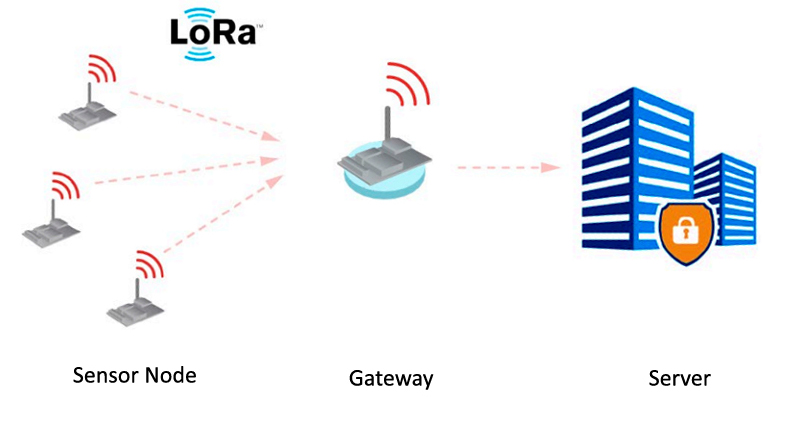
\includegraphics[scale=0.35]{image/normal}
	\end{center}
	\caption{Mô hình hoạt động của mạng}
	\label{normal}
\end{figure}
\end{center}
\par 
Trong trường hợp mạng đang hoạt động bình thường, có một nút mới tham gia vào mạng, nút này sẽ gửi yêu cầu đến Gateway. Sau khi được Gateway chấp nhận thì nút sẽ gửi dữ liệu đến Gateway theo một chu kỳ như những nút khác.
\section{Xây dựng lưu đồ thuật toán xử lý trên STM32}   
Với mô hình truyền thông hình sao như đề xuất trên, module truyền thông SX1278 trên mỗi nút mạng trong hệ thống được điều khiển bởi vi xử lý STM32 thông qua giao tiếp UART. Một số thuật toán điều khiển hoạt động của nút được trình bày trong các phần sau đây. 
\subsection{Gateway} 
 Trong quá trình truyền nhận dữ liệu, Gateway có các chức năng chính sau:
 \begin{itemize}
 \item	Gateway tự động cấu hình,
 \item	Nhận dữ liệu từ các nút,
 \item	Quản lý nút trong mạng.
 \end{itemize}
 \par 
Sau khi đã cấu hình cho gateway, trong vòng lặp vô hạn, gateway liên tục mở kênh truyền để nhận bản tin. Nếu bản tin đó là do một nút mới gửi đến (nút chưa tham gia vào mạng) thì gateway sẽ tiến hành quá trình xác thực nút. Còn nếu bản tin là bản tin chứa dữ liệu, Gateway sẽ nhận và xử lý dữ liệu và tiếp tục quá trình mở kênh truyền để nhận dữ liệu. Thuật toán \ref{gateway} thể hiện thuật toán xử lý của Gateway.
\begin{center}
\begin{algorithm}[h]
	\caption{Thuật toán của Gateway}
	\label{gateway}
	\begin{algorithmic}[1]
		\State $pass \gets sanslab$
		\State Gateway tự động cấu hình  \Comment{Gateway sẽ tự động cài một số thông số như ID, SF, CR, tần số,...}
		\While{1}
			\If{Nhận được gói tin}
				\State $packet \gets packet\_receive$	\Comment{gói tin nhận được}
				\If{$packet$ là gói tin gửi dữ liệu}
					\State $data \gets packet.data$
					\State Xử lý dữ liệu	\Comment{Gateway có thể gửi dữ liệu lên Server, hiển thị hoặc lưu dữ liệu}
				\ElsIf{$packet$ là gói tin yêu cầu tham gia mạng}
					\State	$ID \gets packet.src$	\Comment{Lấy ID của nút gửi đến}
					\State	$authentication \gets packet.data$ \Comment{Lấy dữ liệu bản tin xác thực}
					\State 	$response \gets true$
					\If{$authentication \neq pass$ }
						\State $response \gets flase$
					\EndIf
					\State gửi bản tin phản hồi response cho nút ID
				\EndIf
			\EndIf		
		\EndWhile
	\end{algorithmic}
\end{algorithm}
\end{center}
\subsection{Nút} 
Trong quá trình truyền nhận dữ liệu, nút có các chức năng chính sau:
\begin{itemize}
\item	Nút tự động cấu hình, mỗi nút có một ID khác nhau,
\item	Khi nút chưa tham gia mạng, nút sẽ gửi yêu cầu để tham gia mạng. Khi đó xảy ra một số trường hợp sau:
	\begin{itemize}
	\item	Quá trình yêu cầu không thành công, nút sẽ gửi lại,
	\item	Nếu bản tin xác thực sai, nút sẽ không hoạt động nữa,
	\item	Nếu quá trình yêu cầu tham gia mạng thành công, nút sẽ gửi dữ liệu.
	\end{itemize}
\item	Sau khi tham gia mạng thành công, nút sẽ gửi dữ liệu theo chu kỳ.
\end{itemize}
Sau khi được cấu hình, nút sẽ gửi bản tin xác thực cho Gateway (ID của Gateway được cấu hình sẵn trong nút). Nút sẽ thực hiện quá trình yêu cầu tham gia mạng (\ref{RequestJoinNetworks}) đến khi thành công (nếu bản tin xác thực sai, nút sẽ dừng lại). Sau khi nút nhận được bản tin chấp nhận tham gia vào mạng của Gateway, nút sẽ tiến hành quá trình gửi dữ liệu (quá trình này được thực hiên theo chu kỳ). Quá trình xử lý của nút được thể hiện \ref{node}{}.
\begin{center}
\begin{algorithm}[h]
	\caption{Thuật toán của Nút}
	\label{node}
	\begin{algorithmic}[1]
		\State {$msgAuthentication \gets sanslab$}
		\State Nút tự động cấu hình  \Comment{Nút sẽ tự động cài một số thông số như ID, SF, CR, tần số,...}
		
		\State {$idGateway \gets$ Địa chỉ Gateway}		
		\State {$response \gets 2 $} \Comment{response = 0 --> bản tin xác thực chính xác; response = 1 --> bản tin xác thực không chính xác; response = 2 --> nút chưa tham gia mạng}
		
		\State $RequestJoinNetworks(idGateway, msgAuthentication)$
		
		\While{1}
			\If{$response == 0$}
				\State $data \gets$ lấy dữ liệu từ cảm biến
				\State $cnt = 0$
				\Repeat
					\State $state \gets sendPacket(idGateway, data)$ 
					\If{$state > 0$} 
						\State Delay()
					\EndIf
					\State $cnt \gets cnt + 1$
				\Until{$state > 0$ and $cnt < threshold$} \Comment{threshold là số lần gửi tối đa}
			\ElsIf{$response == 1$} 
				\State $Sleep()$ 
				\Else
					\State $RequestJoinNetworks(idGateway, msgAuthentication)$
				\EndIf
			%\EndIf
		\EndWhile
	\end{algorithmic}
\end{algorithm}
\end{center}
\par 
Trong quá trình yêu cầu tham gia vào mạng, nút sẽ gửi bản tin xác thực đến khi nào nhận lại được bản tin phản hồi của Gateway. Khi đó nút sẽ biết đươc mình đã được chấp thuận tham gia mạng hay chưa. Còn về phần Gateway, sau khi nhận được bản tin xác thực được gửi từ nút, Gateway sẽ kiểm tra bản tin xác thực đó có chính xác không. Kết quả của quá trình kiểm tra bản tin xác thực sẽ được Gateway gửi lại cho nút
\begin{algorithm}
\caption{RequestJoinNetworks}
\label{RequestJoinNetworks}
\begin{algorithmic}[1]
  \Procedure {RequestJoinNetworks}{$idGateway$, $msgAuthentication$}
	\Repeat
			\State $state \gets sendPacket(idGateway, msgAuthentication)$ 
			\Comment{state là trạng thái của quá trình gửi tin; state = 0 gửi bản tin thành công; state > 0 gửi bản tin chưa thành công}
			\If{$state > 0$} 
				\State Delay()
			\ElsIf{Nhận được bản tin hồi đáp từ Gateway}
				\State $response \gets packet\_receive.data$
				\If{$response$ không chính xác} 
					\State $state \gets 1$
				\EndIf
			\EndIf
	\Until{$state > 0$}
  \EndProcedure
\end{algorithmic}
\end{algorithm}
\section{Kết luận}
Trong chương 3, em đã trình bày mô tả giao thức đa truy nhập mà em đã xây dựng để giải quyết đề tài. Sau quá trình xây dựng, triển khai và thí nghiệm, em xin trình bày kết quả đạt được trong chương sau.




\chapter{Phân tích thiết kế hệ thống}
\label{chapter3}
Từ những cơ sở lý thuyết thu thập ở chương \ref{chapter2}, chương \ref{chapter3} em sẽ trình bày phân tích yêu cầu chức năng quy trình thiết kế hệ thống.
\section{Phân tích yêu cầu}
\subsection{Mô tả hệ thống}
Một website thương mại cho phép cửa hàng có thể bán tất cả các loại mặt hàng, có thể giao dịch trực tuyển qua nhiều hinhf thức thanh toán như là: Ngân Lượng, Bảo Kim, ATM, COD,...
Chủ đạo của website là đăng thông tin sản phẩm thật cho khách hàng dễ dàng tìm kiểm thông qua mạng Internet rất phổ cập hiện nay. Người quản trị chính là chủ cửa hàng có một trang quản trị riêng đẻ đăng những thông tin sản phầm, quản lý hoá đơn mua hàng, xem doanh thu theo những mốc thời gian mà người quản trị cần, quản lý thông tin cửa hàng, quản lý quyền cho hệ thống cũng như những tài khoản của khách hàng và cho phép cửa hàng có thể bán thêm những mặt hàng mới nên sẽ phải có hệ thống danh mục sản phầm động. Để thuận tiện cho người quản lý phải có thêm chức năng tìm kiếm ở mỗi chức năng quản lý.
\par
Đối với khách hàng họ cần có 1 tài khoản với thông tin chính xác đề người quản trị liên hệ lại với họ và tiền hành giao dịch mua bán. Với trang chủ để khách hàng xem thông tin sản phẩm chúng ta cần phải có 1 giao diện bắt mắt và thân thiện với người dùng kèm theo đấy là những chức năng tìm kiếm theo những điều kiện khác nhau để người dùng có thể xem những sản phầm họ cần thật nhanh. Vì đây là 1 trang web thương mại điện tử chúng ta không thể thiếu đi được chức năng đăng ký đăng nhập cũng như thay đổi các thông tin cá nhân liên quan đến tài khoản người dùng. Một điều quan trọng hơn nữa là phải lưu được hoá đơn kèm theo đối với mỗi tài khoản người dùng và hỗ trợ chức năng thêm nhiều sản phẩm vào giỏ hàng để người sử dụng dễ dàng hơn trong việc mua sắm.
\subsection{Yêu cầu hệ thống}
\subsubsection{Yêu cầu chức năng}
 Hệ thống website thương mại điện tử sẽ được chia theo nhiều cấp độ người dùng:
\begin{itemize}
 \item Người quản trị: Có mọi quyền để tương tác trong hệ thống, người quản trị có thể thay đối bất kì thông tin của sản phẩm hay đăng bài viết của cửa hàng mình lên tràng chủ, người quản lý có thêm thêm nhân viên giao hàng vào các đơn hàng mà phương thức vận chuyển là COD, người quản lý có thể xem doanh thu bán hàng.  
 \item Nhân viên quản lý của hàng: Chỉ có thế xem và sửa thông tin các sản phầm để cập nhật nhanh chóng lên trang chủ phục vụ nhu cầu của khách hàng.
 \item Người vận chuyển hàng: Chỉ được xem hoá đơn theo trạng thái COD và vận chuyển hàng theo đơn hàng đã được giao trong hệ thống.
 \item Khách hàng: Khách hàng chỉ được phép truy cập ở trang chủ còn trang quản trị thì họ không có quyền gì, khách hàng có thể đăng kí, đăng nhập, và thay đổi thông tin tài khoản để mua hàng, họ cũng có thể gửi những đóng góp cho người quản trị để phát triền website hơn nữa.
\end{itemize}  
\subsubsection{Yêu cầu phi chức năng}
Ngoài các yêu cầu chức năng hệ thống còn có những yêu cầu phi chức năng sau:
\begin{itemize}
\item Hệ thồng có dung lượng không quá lớn, tốc độ xử lý nhanh hơn.
\item Công việc thực hiện chính xác.
\item Sử dụng mã hoá các thông tin nhạy cảm của khách hàng như: mật khẩu, ngày sinh nhật, số điện thoại,...
\item Đảm bảo an toàn dữ liệu khi chạy website trực tuyến
\end{itemize}
\section{Thiết kế hệ thống}
\subsection{Sơ đồ tổng quan hệ thống}
Hệ thống website bao gồm:
\begin{itemize}
    \item Cơ sở dữ liệu là một tập hợp những thông tin được tổ chức để dễ dàng trong việc tạo lập, cập nhập và khai thác thông tin. Cơ sở dữ liệu được duy trì dưới dạng một tập hợp các tập tin trong hệ điều hành hay được lưu trữ trong các hệ quản trị cơ sở dữ liệu. Cơ sở dữ liệu được phân chia thành nhiều loại khác nhau:
   \begin{itemize}
   \item Cơ sở dữ liệu dạng file: dữ liệu được lưu trữ dưới dạng các file có thể là text, ascii,...
   \item Cơ sở dữ liệu quan hệ: dữ liệu được lưu trữ trong các bảng dữ liệu gọi là các thực thể, giữa các thực thể này có mối liên hệ với nhau gọi là các quan hệ, mỗi quan hệ có các thuộc tính, trong đó có một thuộc tính là khóa chính. Các hệ quản trị hỗ trợ cơ sở dữ liệu quan hệ như: MS SQL server, Oracle, MySQL...
   \item Cơ sở dữ liệu hướng đối tượng: dữ liệu cũng được lưu trữ trong các bảng dữ liệu nhưng các bảng có bổ sung thêm các tính năng hướng đối tượng như lưu trữ thêm các hành vi, nhằm thể hiện hành vi của đối tượng. Mỗi bảng xem như một lớp dữ liệu, một dòng dữ liệu trong bảng là một đối tượng. Các hệ quản trị có hỗ trợ cơ sở dữ liệu hướng đối tượng như: MS SQL server, Oracle, Postgres
   \item Cơ sở dữ liệu bán cấu trúc: dữ liệu được lưu dưới dạng XML, với định dạng này thông tin mô tả về đối tượng thể hiện trong các tag. Đây là cơ sở dữ liệu có nhiều ưu điểm do lưu trữ được hầu hết các loại dữ liệu khác nhau nên cơ sở dữ liệu bán cấu trúc là hướng mới trong nghiên cứu và ứng dụng.
   \item Cơ sở dữ liệu phân cấp (blockchain): Dữ liệu được phân tán trên mạng máy tính ngang hàng và luôn được cả mạng lưới kiểm định. Ví dụ: Bitcoin blockchain.
   \end{itemize}
    \item Trang quản trị bao gồm các công việc liên quan đến xử lý nội dung, hình ảnh và các vấn đề phát sinh trong quá trình sử dụng như chữa lỗi, bảo mật, sao lưu và phục hồi thông tin.
    \item Trang chủ website, hiện nay có 2 loại trang chủ website là: 
    \begin{itemize}
    \item Website tĩnh là website mà người quản trị (những người không phải là lập trình viên) không thể tùy ý thay đổi nội dung và hình ảnh mà phải cần kiến thức về HTML cơ bản. Website tĩnh được viết hoàn toàn dựa trên nền tảng HTML CSS và thêm các hiệu ứng từ Javascript nếu muốn.
    \item Website động là website được viết kèm theo một bộ công cụ quản trị để tùy biến nội dung dành cho webmaster (người quản trị) có thể dễ dàng thay đổi nội dung, hình ảnh. Website động được thiết kế bởi các lập trình viên để làm sao cho phép website có thể thay đổi được nội dung thường xuyên. Một số công nghệ, ngôn ngữ để xây dựng website động bao gồm PHP, ASP.NET, Java,...
    \end{itemize}
\end{itemize}
\begin{center}
    \begin{figure}[h]
    \begin{center}
     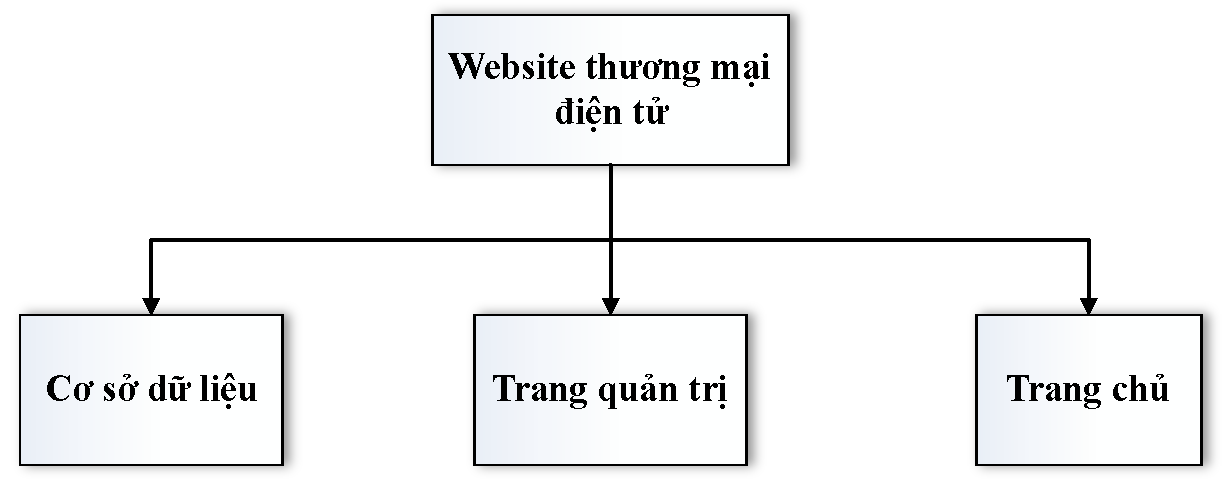
\includegraphics[scale=0.7]{image/TongQuanHeThong.pdf}
    \end{center}
    \caption{Tổng Quan Hệ thống}
    \label{refhinh3_1}
    \end{figure}
\end{center}
\subsection{Sơ đồ Use case diagram}
Một biểu đồ Use case chỉ ra một số lượng các tác nhân ngoại cảnh và mối liên
kết của chúng đối với Use case mà hệ thống cung cấp. Một Use case là một lời miêu tả của một chức năng mà hệ thống cung cấp. Lời miêu tả Use case thường là một văn bản tài liệu, nhưng kèm theo đó cũng có thể là một biểu đồ hoạt động. Các Use case được miêu tả duy nhất theo hướng nhìn từ ngoài vào của các tác nhân (hành vi của hệ thống theo như sự mong đợi của người sử dụng), không miêu tả chức năng được cung cấp sẽ hoạt động nội bộ bên trong hệ thống ra sao. Các Use case định nghĩa các yêu cầu về mặt chức năng đối với hệ thống.
\subsubsection{Quản Trị Viên}
Quản trị viên có vai trò cao nhất trong hệ thống có thể truy cập bất cứ chức năng gì trong hệ thống. Quản trị viên có những chức năng sau:
\begin{itemize}
 \item Tạo ra tài khoản cho các cấp người dùng.
 \item Tạo ra các quyền và nhóm quyền sau đó gán cho người dùng tương ứng.
 \item Thêm, sửa, xoá, xem thông tin sản phẩm, danh mục sản phẩm, hoá đơn bán hàng, người vận chuyển, những quảng cáo trên website, góp ý khách hàng, thông tin của cửa hàng.
 \item Khoá một tài khoản của người dùng.
 \item Xem doanh thu của cửa hàng.
 \item Gửi mail cho người dùng sau khi người dùng đăng kí tài khoản.
 \item Được xem hiển thị thông báo mỗi khi hệ thống có sự thay đổi như: thêm mới, sửa, xoá, hay có một đơn hàng mới.
 \end{itemize}
\newpage
 \begin{center}
    \begin{figure}[h]
    \begin{center}
     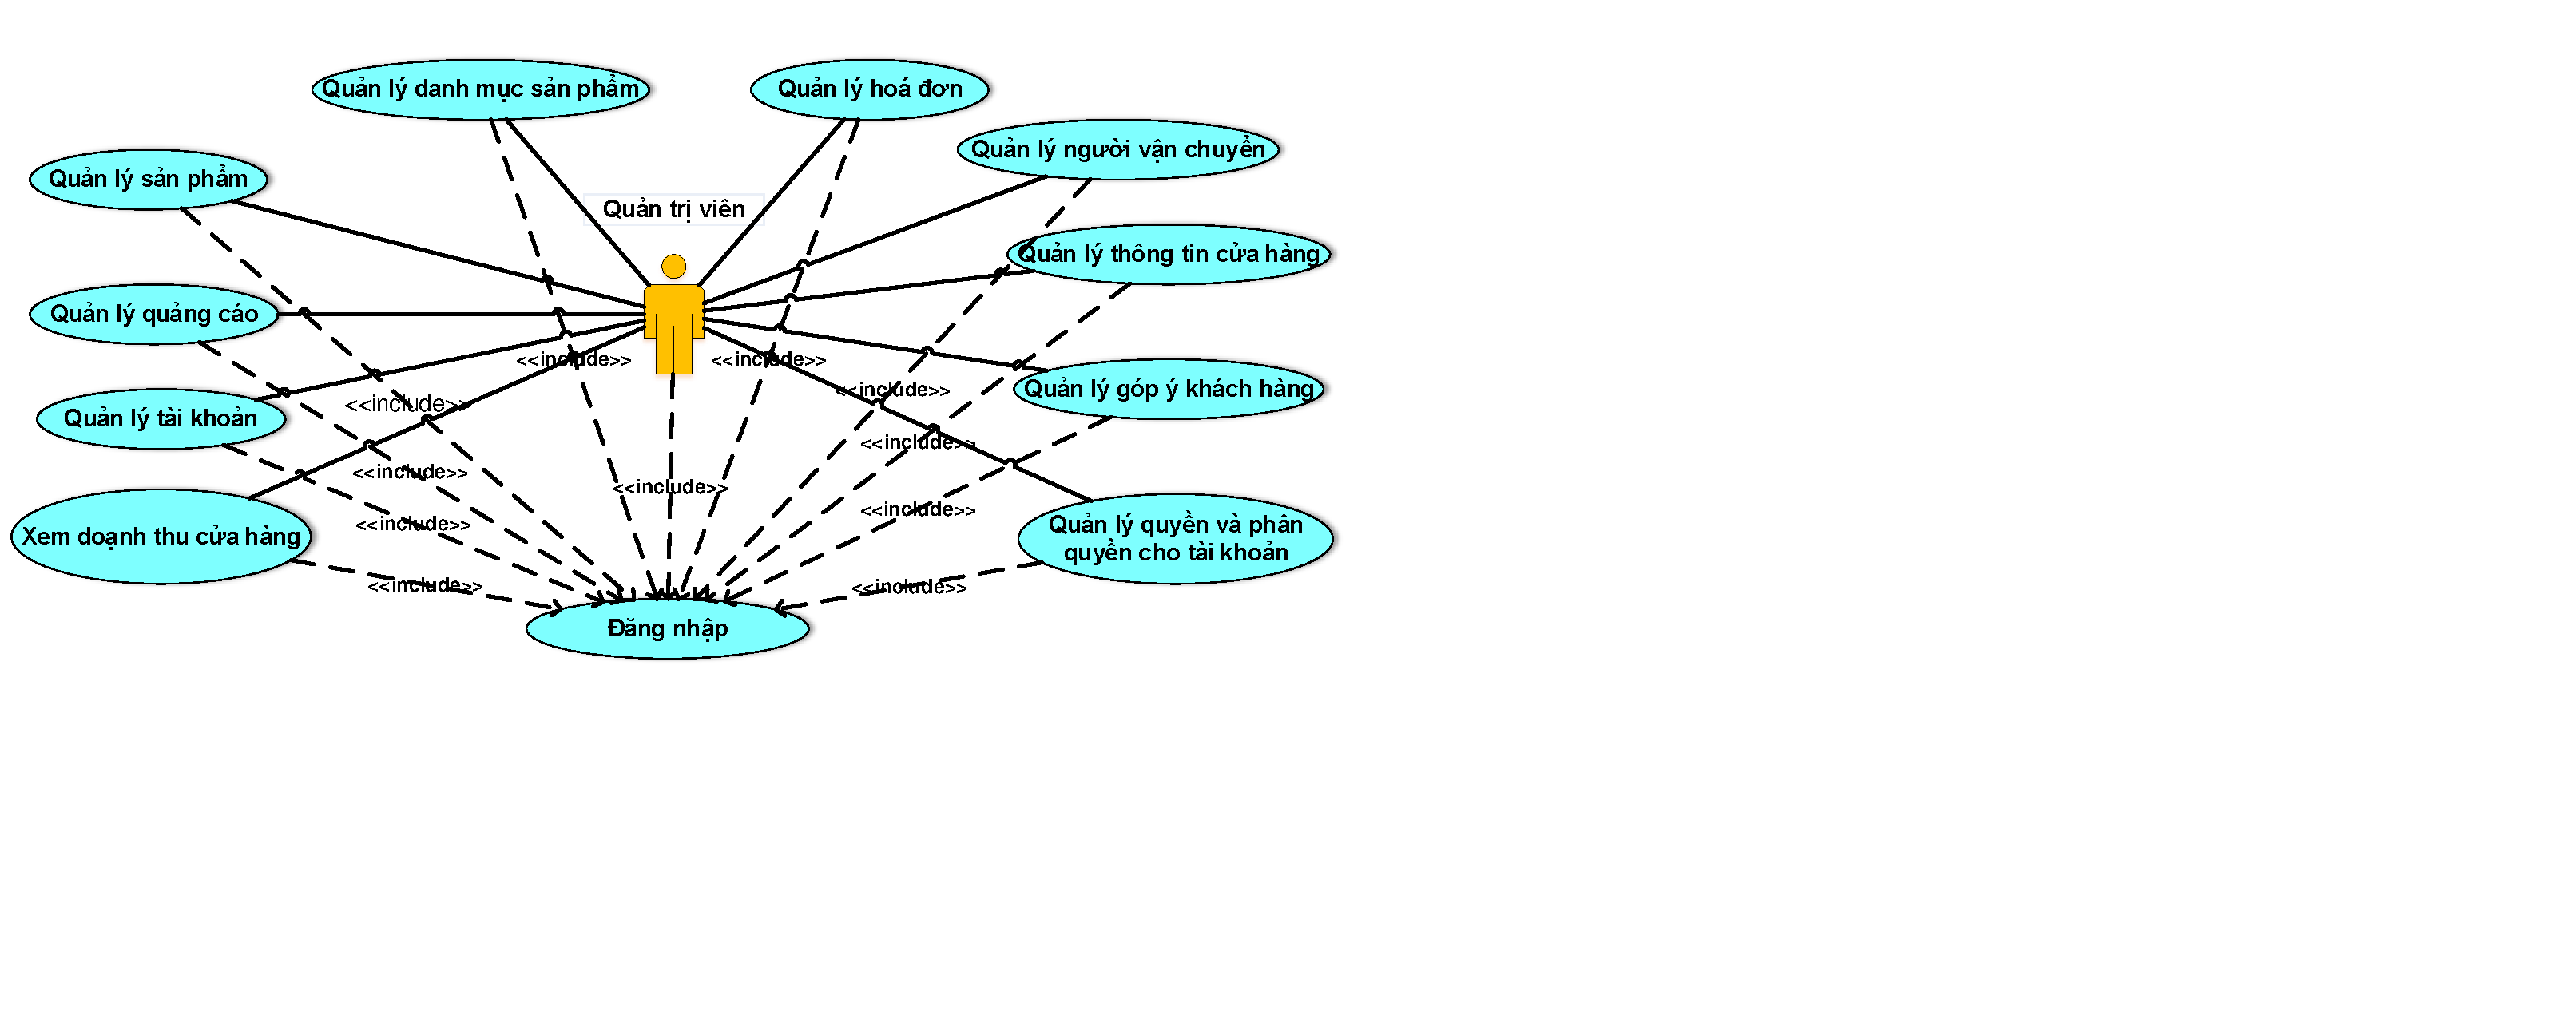
\includegraphics[scale=0.5]{image/UseCaseTongQuanQTV.pdf}
    \end{center}
    \caption{Use-Case Quản Trị Viên}
    \label{refhinh3_2}
    \end{figure}
\end{center}
Từ Hình \ref{refhinh3_2} ta có các bảng đặc tả chi tiết cho các Use-Case của quản trị viên:
- Use-Case đăng nhập:
\begin{longtable}[htp]{ |m{0.25\linewidth}|m{0.65\linewidth}|}
 \caption{Bảng Use-Case đăng nhập \label{login}}\\
 \hline
 Use-Case & Nội dung \\
 \hline
 Tên Use-Case & Đăng nhập \\
 \hline
 Mô tả & Use-case cho phép quản trị viên đăng nhập vào hệ thống để thực hiện những chức năng của mình\\
 \hline
 Tên tác nhân & Quản trị viên\\
 \hline
 Điều kiện kích hoạt & Quản trị viên vào trang admin trên hệ thống, trang admin bắt buộc phải đăng nhập\\
 \hline
 Tiền điều kiện & Quản trị viên phải có tài khoản trên hệ thống và được phân quyền quản trị viên\\
 \hline
 Hậu điều kiện & Quản trị viên đăng nhập thành công\\
 \hline
 Luồng sự kiện chính & 
  1. Hệ thống hiện thị màn hình đăng nhập.\newline
  2. Quản trị viên nhập tên đăng nhập và mật khẩu.\newline
  3. Hệ thống kiểm tra thông tin đăng nhập và kiểm qua quyền của tài khoản là admin.\newline
  4. Nếu thành công hệ thống sẽ đưa quản trị viên vào trang chủ của trang quản trị.\newline
  5. Kết thúc Use-case.	
 \\
 \hline
 Luồng sự kiện phụ & 
 - Tài khoản và mật khẩu không hợp lệ:\newline
 1. Khi quản trị viên nhập sai tên đăng nhập và mật khẩu\newline
 2. Hệ thống hiển thị lại màn hình đăng nhập để quản trị viên nhập lại thông tin tài khoản và mật khẩu kèm theo thông báo tên đăng nhập và mật khẩu bị sai.\newline
  Quay lại bước 2 trong luồng sự kiện chính.
 \\
 \hline
\end{longtable}
\par
- Use-Case Đăng xuất:

\begin{longtable}[htp]{ |m{0.3\linewidth}|m{0.6\linewidth}|}
 \caption{Bảng Use-Case đăng xuất \label{logout}}\\
 \hline
 Use-Case & Nội dung \\
 \hline
 Tên Use-Case & Đăng xuất \\
 \hline
 Mô tả & Use-case cho phép quản trị viên đăng xuất ra khỏi hệ thống\\
 \hline
 Tên tác nhân & Quản trị viên\\
 \hline
 Điều kiện kích hoạt & Quản trị viên nhấn nút đăng xuất trên màn hình hệ thống\\
 \hline
 Tiền điều kiện & Quản trị viên đã đăng nhập vào hệ thống\\
 \hline
 Hậu điều kiện & Quản trị viên đăng xuất thành công\\
 \hline
 Luồng sự kiện chính & 
 1. Quản trị viên tìm và nhấn nút đăng xuất.\newline
 2. Hệ thống xử lý yêu cầu đăng xuất của quản trị viên.\newline
 3. Kết thúc Use-case.	
 \\
 \hline
\end{longtable}

- Use-case quản lý tài khoản:

\begin{longtable}[htp]{ |m{0.3\linewidth}|m{0.6\linewidth}|}
 \caption{Bảng Use-Case thêm mới tài khoản \label{long}}\\
 \hline
 Use-Case & Nội dung \\
 \hline
 Tên Use-Case & Thêm mới tài khoản \\
 \hline
 Mô tả & Use-case cho phép quản trị viên thêm mới tài khoản để cấp cho người dùng sử dụng hệ thống\\
 \hline
 Tên tác nhân & Quản trị viên\\
 \hline
 Điều kiện kích hoạt & Quản trị viên vào trang admin trên hệ thống, chọn chức năng thêm tài khoản\\
 \hline
 Tiền điều kiện & Quản trị viên phải đăng nhập vào hệ thống và có quyền thêm tài khoản\\
 \hline
 Hậu điều kiện & Thông tin tài khoản mới được cập nhật vào cơ sở dữ liệu\\
 \hline
 Luồng sự kiện chính & 
 1. Quản trị viên kích hoạt yêu cầu thêm tài khoản.\newline
 2. Hệ thống hiển thị giao diện thêm tài khoản và yêu cầu quản trị viên nhập thông tin tài khoản.\newline
 3. Quản trị viên nhâp thông tin tài khoản mới và nhấn lưu tài khoản.\newline
 4. Hệ thống kiểm tra thông tin tài khoản và xác nhận hợp lệ.\newline
 5. Hệ thống thông báo đã lưu thành công tài khoản.\newline	
 6. Quản trị viên thoát khỏi chức năng thêm tài khoản
 \\
 \hline
 Luồng sự kiện phụ & 
 - Dữ liệu không đúng:\newline
  1. Hệ thống hiển thị lại giao diện nhập thông tin tài khoản để quản trị viên nhập lại đồng thời hiện thị thông báo lưu tài khoản không thành công.\newline
  2. Quay lại bước 2 của luồng sự kiện chính.\newline
  - Không có quyền thực hiện chức năng:\newline
  1. Hệ thống kiểm tra lúc đăng nhập tài khoản không có quyền thực hiện chức năng.\newline
  2. Trên thanh chức năng không có chức năng thêm tài khoản
 \\
 \hline
\end{longtable}

\begin{longtable}[htp]{ |m{0.3\linewidth}|m{0.6\linewidth}|}
 \caption{Bảng Use-Case sửa tài khoản \label{long}}\\
 \hline
 Use-Case & Nội dung \\
 \hline
 Tên Use-Case & Sửa tài khoản \\
 \hline
 Mô tả & Use-case cho phép quản trị viên sửa tài khoản cho người sử dụng hệ thống\\
 \hline
 Tên tác nhân & Quản trị viên\\
 \hline
 Điều kiện kích hoạt & Quản trị viên vào trang admin trên hệ thống, chọn 1 tài khoản trong danh sách tài khoản\\
 \hline
 Tiền điều kiện & Quản trị viên phải đăng nhập vào hệ thống và có quyền sửa tài khoản\\
 \hline
 Hậu điều kiện & Thông tin tài khoản sau khi sửa được cập nhật vào cơ sở dữ liệu\\
 \hline
 Luồng sự kiện chính & 
 1. Quản trị viên chọn 1 tài khoản.
 2. Quản trị viên kích hoạt yêu cầu sửa tài khoản.\newline
 3. Hệ thống hiển thị giao diện sửa tài khoản và những thông tin tài khoản đã được chọn, yêu cầu quản trị viên sửa tài khoản.\newline
 4. Quản trị viên nhâp thông tin tài khoản mới và nhấn lưu tài khoản.\newline
 5. Hệ thống kiểm tra thông tin tài khoản và xác nhận hợp lệ.\newline
 6. Hệ thống thông báo đã lưu thành công tài khoản.\newline	
 7. Quản trị viên thoát khỏi chức năng sửa tài khoản
 \\
 \hline
 Luồng sự kiện phụ & 
 - Dữ liệu không đúng:\newline
  1. Hệ thống hiển thị lại giao diện nhập thông tin tài khoản để quản trị viên nhập lại đồng thời hiện thị thông báo lưu tài khoản không thành công.\newline
  2. Quay lại bước 2 của luồng sự kiện chính.\newline
  - Không có quyền thực hiện chức năng:\newline
  1. Hệ thống kiểm tra lúc đăng nhập tài khoản không có quyền thực hiện chức năng.\newline
  2. Trên thanh chức năng không có chức năng sửa tài khoảm
 \\
 \hline
\end{longtable}

\begin{longtable}[htp]{ |m{0.3\linewidth}|m{0.6\linewidth}|}
 \caption{Bảng Use-Case xoá tài khoản \label{long}}\\
 \hline
 Use-Case & Nội dung \\
 \hline
 Tên Use-Case & Xoá tài khoản \\
 \hline
 Mô tả & Use-case cho phép quản trị viên xoá tài khoản khi người dùng không sử dụng\\
 \hline
 Tên tác nhân & Quản trị viên\\
 \hline
 Điều kiện kích hoạt & Quản trị viên vào trang admin trên hệ thống, chọn 1 tài khoản trong danh sách tài khoản\\
 \hline
 Tiền điều kiện & Quản trị viên phải đăng nhập vào hệ thống và có quyền xoá tài khoản\\
 \hline
 Hậu điều kiện & Thông tin tài khoản đã chọn được xoá khỏi cơ sở dữ liệu\\
 \hline
 Luồng sự kiện chính & 
 1. Quản trị viên chọn 1 tài khoản.
 2. Quản trị viên kích hoạt yêu cầu xoá tài khoản.\newline
 3. Hệ thống hiển thị giao diện xoá tài khoản và yêu cầu quản trị viên xác nhận có đồng ý xoá không.\newline
 4. Quản trị viên chọn có trên màn hình giao diện.\newline
 5. Hệ thống xoá tài khoản khỏi cơ sở dữ liệu.\newline
 6. Hệ thống thông báo đã xoá thành công tài khoản.\newline	
 7. Quản trị viên thoát khỏi chức năng xoá tài khoản
 \\
 \hline
 Luồng sự kiện phụ & 
 - Không có quyền thực hiện chức năng:\newline
  1. Hệ thống kiểm tra lúc đăng nhập tài khoản không có quyền thực hiện chức năng.\newline
  2. Trên thanh chức năng không có chức năng xoá tài khoảm
 \\
 \hline
\end{longtable}

- Quản lý sản phẩm:
\begin{longtable}[htp]{ |m{0.3\linewidth}|m{0.6\linewidth}|}
 \caption{Bảng Use-Case thêm sản phẩm \label{createProduct}}\\
 \hline
 Use-Case & Nội dung \\
 \hline
 Tên Use-Case & Thêm sản phẩm \\
 \hline
 Mô tả & Use-case cho phép quản trị viên thêm sản phẩm để hiển thị trên trang chủ\\
 \hline
 Tên tác nhân & Quản trị viên\\
 \hline
 Điều kiện kích hoạt & Quản trị viên vào trang admin trên hệ thống, chọn chức năng thêm sản phẩm\\
 \hline
 Tiền điều kiện & Quản trị viên phải đăng nhập vào hệ thống và có quyền thêm sản phẩm\\
 \hline
 Hậu điều kiện & Thông tin sản phẩm sau khi thêm mới được cập nhật vào cơ sở dữ liệu\\
 \hline
 Luồng sự kiện chính & 
 1. Quản trị viên kích hoạt yêu cầu thêm sản phẩm.\newline
 2. Hệ thống hiển thị giao diện thêm sản phẩm và yêu cầu quản trị viên nhập thông tin sản phẩm.\newline
 3. Quản trị viên nhâp thông tin sản phẩm mới bao gồm: giá, tải ảnh sản phẩm, tên sản phẩm,... và nhấn lưu sản phẩm.\newline
 4. Hệ thống kiểm tra thông tin sản phẩm và xác nhận hợp lệ.\newline
 5. Hệ thống thông báo đã lưu thành công sản phẩm.\newline	
 6. Quản trị viên thoát khỏi chức năng thêm sản phẩm.
 \\
 \hline
 Luồng sự kiện phụ & 
 - Dữ liệu không đúng:\newline
  1. Hệ thống hiển thị lại giao diện nhập thông tin sản phẩm để quản trị viên nhập lại đồng thời hiện thị thông báo lưu sản phẩm không thành công.\newline
  2. Quay lại bước 2 của luồng sự kiện chính.\newline
  - Không có quyền thực hiện chức năng:\newline
  1. Hệ thống kiểm tra lúc đăng nhập tài khoản không có quyền thực hiện chức năng.\newline
  2. Trên thanh chức năng không có chức năng thêm sản phẩm.
 \\
 \hline
\end{longtable}

\begin{longtable}[htp]{ |m{0.3\linewidth}|m{0.6\linewidth}|}
 \caption{Bảng Use-Case sửa sản phẩm \label{updateProduct}}\\
 \hline
 Use-Case & Nội dung \\
 \hline
 Tên Use-Case & Sửa sản phẩm \\
 \hline
 Mô tả & Use-case cho phép quản trị viên sửa sản phẩm để hiển thị trên trang chủ\\
 \hline
 Tên tác nhân & Quản trị viên\\
 \hline
 Điều kiện kích hoạt & Quản trị viên vào trang admin trên hệ thống, chọn chức năng sửa sản phẩm\\
 \hline
 Tiền điều kiện & Quản trị viên phải đăng nhập vào hệ thống và có quyền sửa sản phẩm\\
 \hline
 Hậu điều kiện & Thông tin sản phẩm sau khi sửa được cập nhật vào cơ sở dữ liệu\\
 \hline
 Luồng sự kiện chính & 
 1. Quản trị viên chọn 1 trong số sản phẩm cần sửa trong danh sách sản phẩm.
 2. Quản trị viên kích hoạt yêu cầu sửa sản phẩm.\newline
 3. Hệ thống hiển thị giao diện sửa sản phẩm đồng thời hiển thị các thông tin của sản phẩm được chọn và yêu cầu quản trị viên nhập thông tin sản phẩm cần sửa.\newline
 4. Quản trị viên nhâp thông tin sản phẩm mới bao gồm: giá, ảnh sản phẩm, tên sản phẩm,... và nhấn lưu sản phẩm.\newline
 5. Hệ thống kiểm tra thông tin sản phẩm và xác nhận hợp lệ.\newline
 6. Hệ thống thông báo đã lưu thành công sản phẩm.\newline	
 7. Quản trị viên thoát khỏi chức năng sửa sản phẩm.
 \\
 \hline
 Luồng sự kiện phụ & 
 - Dữ liệu không đúng:\newline
  1. Hệ thống hiển thị lại giao diện nhập thông tin sản phẩm để quản trị viên nhập lại đồng thời hiện thị thông báo lưu sản phẩm không thành công.\newline
  2. Quay lại bước 2 của luồng sự kiện chính.\newline
  - Không có quyền thực hiện chức năng:\newline
  1. Hệ thống kiểm tra lúc đăng nhập tài khoản không có quyền thực hiện chức năng.\newline
  2. Trên thanh chức năng không có chức năng sửa sản phẩm.
 \\
 \hline
\end{longtable}

\begin{longtable}[htp]{ |m{0.3\linewidth}|m{0.6\linewidth}|}
 \caption{Bảng Use-Case xoá sản phẩm \label{long}}\\
 \hline
 Use-Case & Nội dung \\
 \hline
 Tên Use-Case & Xoá sản phẩm \\
 \hline
 Mô tả & Use-case cho phép quản trị viên xoá sản phẩm\\
 \hline
 Tên tác nhân & Quản trị viên\\
 \hline
 Điều kiện kích hoạt & Quản trị viên vào trang admin trên hệ thống, chọn chức năng xoá sản phẩm\\
 \hline
 Tiền điều kiện & Quản trị viên phải đăng nhập vào hệ thống và có quyền xoá sản phẩm\\
 \hline
 Hậu điều kiện & Thông tin sản phẩm sau khi xoá được cập nhật vào cơ sở dữ liệu\\
 \hline
 Luồng sự kiện chính & 
 1. Quản trị viên chọn 1 trong số sản phẩm cần xoá trong danh sách sản phẩm.
 2. Quản trị viên kích hoạt yêu cầu xoá sản phẩm.\newline
 3. Hệ thống hiển thị giao diện xoá sản phẩm đồng thời hiển thị thông báo có muốn xoá hay không.\newline
 4. Quản trị viên chọn có.\newline
 5. Hệ thống xử lý và thực hiện xoá sản phẩm.\newline
 6. Hệ thống thông báo đã xoá thành công sản phẩm.\newline	
 7. Quản trị viên thoát khỏi chức năng xoá sản phẩm.
 \\
 \hline
 Luồng sự kiện phụ & 
  - Không có quyền thực hiện chức năng:\newline
  1. Hệ thống kiểm tra lúc đăng nhập tài khoản không có quyền thực hiện chức năng.\newline
  2. Trên thanh chức năng không có chức năng xoá sản phẩm.
 \\
 \hline
\end{longtable}

- Quản lý danh mục sản phẩm:
\begin{longtable}[htp]{ |m{0.3\linewidth}|m{0.6\linewidth}|}
 \caption{Bảng Use-Case thêm danh mục sản phẩm \label{long}}\\
 \hline
 Use-Case & Nội dung \\
 \hline
 Tên Use-Case & Thêm danh mục sản phẩm \\
 \hline
 Mô tả & Use-case cho phép quản trị viên thêm danh mục sản phẩm để của hàng có thể bán nhiều mặt hàng\\
 \hline
 Tên tác nhân & Quản trị viên\\
 \hline
 Điều kiện kích hoạt & Quản trị viên vào trang admin trên hệ thống, chọn chức năng thêm danh mục sản phẩm\\
 \hline
 Tiền điều kiện & Quản trị viên phải đăng nhập vào hệ thống và có quyền thêm danh mục sản phẩm\\
 \hline
 Hậu điều kiện & Thông tin danh mục sản phẩm sau khi thêm mới được cập nhật vào cơ sở dữ liệu\\
 \hline
 Luồng sự kiện chính & 
 1. Quản trị viên kích hoạt yêu cầu thêm danh mục sản phẩm.\newline
 2. Hệ thống hiển thị giao diện thêm danh mục sản phẩm và yêu cầu quản trị viên nhập thông tin sản phẩm.\newline
 3. Quản trị viên nhâp thông tin sản phẩm mới bao gồm: tên danh mục, tải ảnh mô tả danh mục sản phẩm,... và nhấn lưu sản phẩm.\newline
 4. Hệ thống kiểm tra thông tin danh mục sản phẩm và xác nhận hợp lệ.\newline
 5. Hệ thống thông báo đã lưu thành công danh mục sản phẩm.\newline	
 6. Quản trị viên thoát khỏi chức năng thêm danh mục sản phẩm.
 \\
 \hline
 Luồng sự kiện phụ & 
 - Dữ liệu không đúng:\newline
  1. Hệ thống hiển thị lại giao diện nhập thông tin danh mục sản phẩm để quản trị viên nhập lại đồng thời hiện thị thông báo lưu danh mục sản phẩm không thành công.\newline
  2. Quay lại bước 2 của luồng sự kiện chính.\newline
  - Không có quyền thực hiện chức năng:\newline
  1. Hệ thống kiểm tra lúc đăng nhập tài khoản không có quyền thực hiện chức năng.\newline
  2. Trên thanh chức năng không có chức năng thêm danh mục sản phẩm.
 \\
 \hline
\end{longtable}

\begin{longtable}[htp]{ |m{0.3\linewidth}|m{0.6\linewidth}|}
 \caption{Bảng Use-Case sửa danh mục sản phẩm \label{long}}\\
 \hline
 Use-Case & Nội dung \\
 \hline
 Tên Use-Case & Sửa danh mục sản phẩm \\
 \hline
 Mô tả & Use-case cho phép quản trị viên sửa danh mục sản phẩm.\\
 \hline
 Tên tác nhân & Quản trị viên\\
 \hline
 Điều kiện kích hoạt & Quản trị viên vào trang admin trên hệ thống, chọn chức năng sửa danh mục sản phẩm\\
 \hline
 Tiền điều kiện & Quản trị viên phải đăng nhập vào hệ thống và có quyền sửa danh mục sản phẩm\\
 \hline
 Hậu điều kiện & Thông tin danh mục sản phẩm sau khi sửa được cập nhật vào cơ sở dữ liệu\\
 \hline
 Luồng sự kiện chính & 
 1. Quản trị viên chọn 1 trong số danh mục sản phẩm cần sửa trong danh sách danh mục sản phẩm.
 2. Quản trị viên kích hoạt yêu cầu sửa danh mục sản phẩm.\newline
 3. Hệ thống hiển thị giao diện sửa danh mục sản phẩm đồng thời hiển thị các thông tin của danh mục sản phẩm được chọn và yêu cầu quản trị viên nhập thông tin danh mục sản phẩm cần sửa.\newline
 4. Quản trị viên nhâp thông tin sản phẩm mới bao gồm: tên danh mục, ảnh mô tả, danh mục cha,... và nhấn lưu danh mục sản phẩm.\newline
 5. Hệ thống kiểm tra thông tin danh mục sản phẩm và xác nhận hợp lệ.\newline
 6. Hệ thống thông báo đã lưu thành công danh mục sản phẩm.\newline	
 7. Quản trị viên thoát khỏi chức năng sửa danh mục sản phẩm.
 \\
 \hline
 Luồng sự kiện phụ & 
 - Dữ liệu không đúng:\newline
  1. Hệ thống hiển thị lại giao diện nhập thông tin sản phẩm để quản trị viên nhập lại đồng thời hiện thị thông báo lưu danh mục sản phẩm không thành công.\newline
  2. Quay lại bước 2 của luồng sự kiện chính.\newline
  - Không có quyền thực hiện chức năng:\newline
  1. Hệ thống kiểm tra lúc đăng nhập tài khoản không có quyền thực hiện chức năng.\newline
  2. Trên thanh chức năng không có chức năng sửa danh mục sản phẩm.
 \\
 \hline
\end{longtable}

\begin{longtable}[htp]{ |m{0.3\linewidth}|m{0.6\linewidth}|}
 \caption{Bảng Use-Case xoá danh mục sản phẩm \label{long}}\\
 \hline
 Use-Case & Nội dung \\
 \hline
 Tên Use-Case & Xoá danh mục sản phẩm \\
 \hline
 Mô tả & Use-case cho phép quản trị viên xoá danh mục sản phẩm\\
 \hline
 Tên tác nhân & Quản trị viên\\
 \hline
 Điều kiện kích hoạt & Quản trị viên vào trang admin trên hệ thống, chọn chức năng xoá danh mục sản phẩm\\
 \hline
 Tiền điều kiện & Quản trị viên phải đăng nhập vào hệ thống và có quyền xoá danh mục sản phẩm\\
 \hline
 Hậu điều kiện & Thông tin danh mục sản phẩm sau khi xoá được cập nhật vào cơ sở dữ liệu\\
 \hline
 Luồng sự kiện chính & 
 1. Quản trị viên chọn 1 trong số danh mục sản phẩm cần xoá trong danh sách danh mục sản phẩm.
 2. Quản trị viên kích hoạt yêu cầu xoá danh mục sản phẩm.\newline
 3. Hệ thống hiển thị giao diện xoá danh mục sản phẩm đồng thời hiển thị thông báo có muốn xoá hay không.\newline
 4. Quản trị viên chọn có.\newline
 5. Hệ thống xử lý và thực hiện xoá danh mục sản phẩm.\newline
 6. Hệ thống thông báo đã xoá thành công danh mục sản phẩm.\newline	
 7. Quản trị viên thoát khỏi chức năng xoá sản phẩm.
 \\
 \hline
 Luồng sự kiện phụ & 
  - Không có quyền thực hiện chức năng:\newline
  1. Hệ thống kiểm tra lúc đăng nhập tài khoản không có quyền thực hiện chức năng.\newline
  2. Trên thanh chức năng không có chức năng xoá danh mục sản phẩm.
 \\
 \hline
\end{longtable}

-Quản lý đơn hàng sản phẩm:
\begin{longtable}[htp]{ |m{0.3\linewidth}|m{0.6\linewidth}|}
 \caption{Bảng Use-Case xem đơn hàng đã được đặt \label{listBill}}\\
 \hline
 Use-Case & Nội dung \\
 \hline
 Tên Use-Case & Xem đơn hàng đã được đặt \\
 \hline
 Mô tả & Use-case cho phép quản trị viên xem các đơn hàng mà khách hàng đã đặt từ trang chủ để xử lý\\
 \hline
 Tên tác nhân & Quản trị viên\\
 \hline
 Điều kiện kích hoạt & Quản trị viên vào trang admin trên hệ thống, chọn chức năng xem đơn hàng\\
 \hline
 Tiền điều kiện & Quản trị viên phải đăng nhập vào hệ thống và có quyền xem các đơn hàng\\
 \hline
 Hậu điều kiện & Hiển thị thành công danh sách đơn hàng từ cơ sở dữ liệu lên màn hình người dùng\\
 \hline
 Luồng sự kiện chính & 
 1. Quản trị viên kích hoạt yêu cầu xem đơn hàng.\newline
 2. Hệ thống xử lý và thực hiện truy vần dữ liệu từ cơ sở dữ liệu gửi lên màn hình người dùng.\newline
 3. Hệ thống hiển thị các đơn hàng đã có từ cơ sở dữ liệu lên màn hình người dùng.\newline	
 4. Quản trị viên thoát khỏi chức năng xem đơn hàng.
 \\
 \hline
 Luồng sự kiện phụ & 
  - Không có quyền thực hiện chức năng:\newline
  1. Hệ thống kiểm tra lúc đăng nhập tài khoản không có quyền thực hiện chức năng.\newline
  2. Trên thanh chức năng không có chức năng xem hoá đơn.
 \\
 \hline
\end{longtable}

\begin{longtable}[htp]{ |m{0.3\linewidth}|m{0.6\linewidth}|}
 \caption{Bảng Use-Case giao đơn hàng đến người vận chuyển \label{long}}\\
 \hline
 Use-Case & Nội dung \\
 \hline
 Tên Use-Case & Giao đơn hàng đến người vận chuyển \\
 \hline
 Mô tả & Use-case cho phép quản trị viên có thể sửa đơn hàng và giao đơn hàng đến người vận chuyển\\
 \hline
 Tên tác nhân & Quản trị viên\\
 \hline
 Điều kiện kích hoạt & Quản trị viên vào trang admin trên hệ thống, chọn chức năng sửa đơn hàng\\
 \hline
 Tiền điều kiện & Quản trị viên phải đăng nhập vào hệ thống và có quyền sửa đơn hàng\\
 \hline
 Hậu điều kiện & Thông tin đơn hàng được lưu vào cơ sở dữ liệu thành công\\
 \hline
 Luồng sự kiện chính & 
 1. Quản trị viên chọn một đơn hàng cần giao đến người vận chuyển.\newline
 2. Hệ thống hiển thị giao diện sửa đơn hàng đồng thời hiển thị các thông tin của đơn hàng được chọn và yêu cầu quản trị viên nhập thông tin đơn hàng cần sửa.\newline
 3. Quản trị viên nhập thông tin đơn hàng cần sửa đặc biệt là thông tin đến người vận chuyển.\newline	
 4. Hệ thống kiểm tra thông tin đơn hàng và xác nhận hợp lệ.
 5. Hệ thống xử lý và thông báo lưu thành công đơn hàng.
 6. Quản trị viên thoát khỏi chắc năng sửa đơn hàng.
 \\
 \hline
 Luồng sự kiện phụ & 
 - Dữ liệu không đúng:\newline
  1. Hệ thống hiển thị lại giao diện nhập thông tin đơn hàng để quản trị viên nhập lại đồng thời hiện thị thông báo lưu đơn hàng không thành công.\newline
  2. Quay lại bước 2 của luồng sự kiện chính.\newline
  - Không có quyền thực hiện chức năng:\newline
  1. Hệ thống kiểm tra lúc đăng nhập tài khoản không có quyền thực hiện chức năng.\newline
  2. Trên thanh chức năng không có chức năng sửa hoá đơn.
 \\
 \hline
\end{longtable}
\newpage
\subsubsection{Khách hàng}
\begin{center}
    \begin{figure}[h]
    \begin{center}
     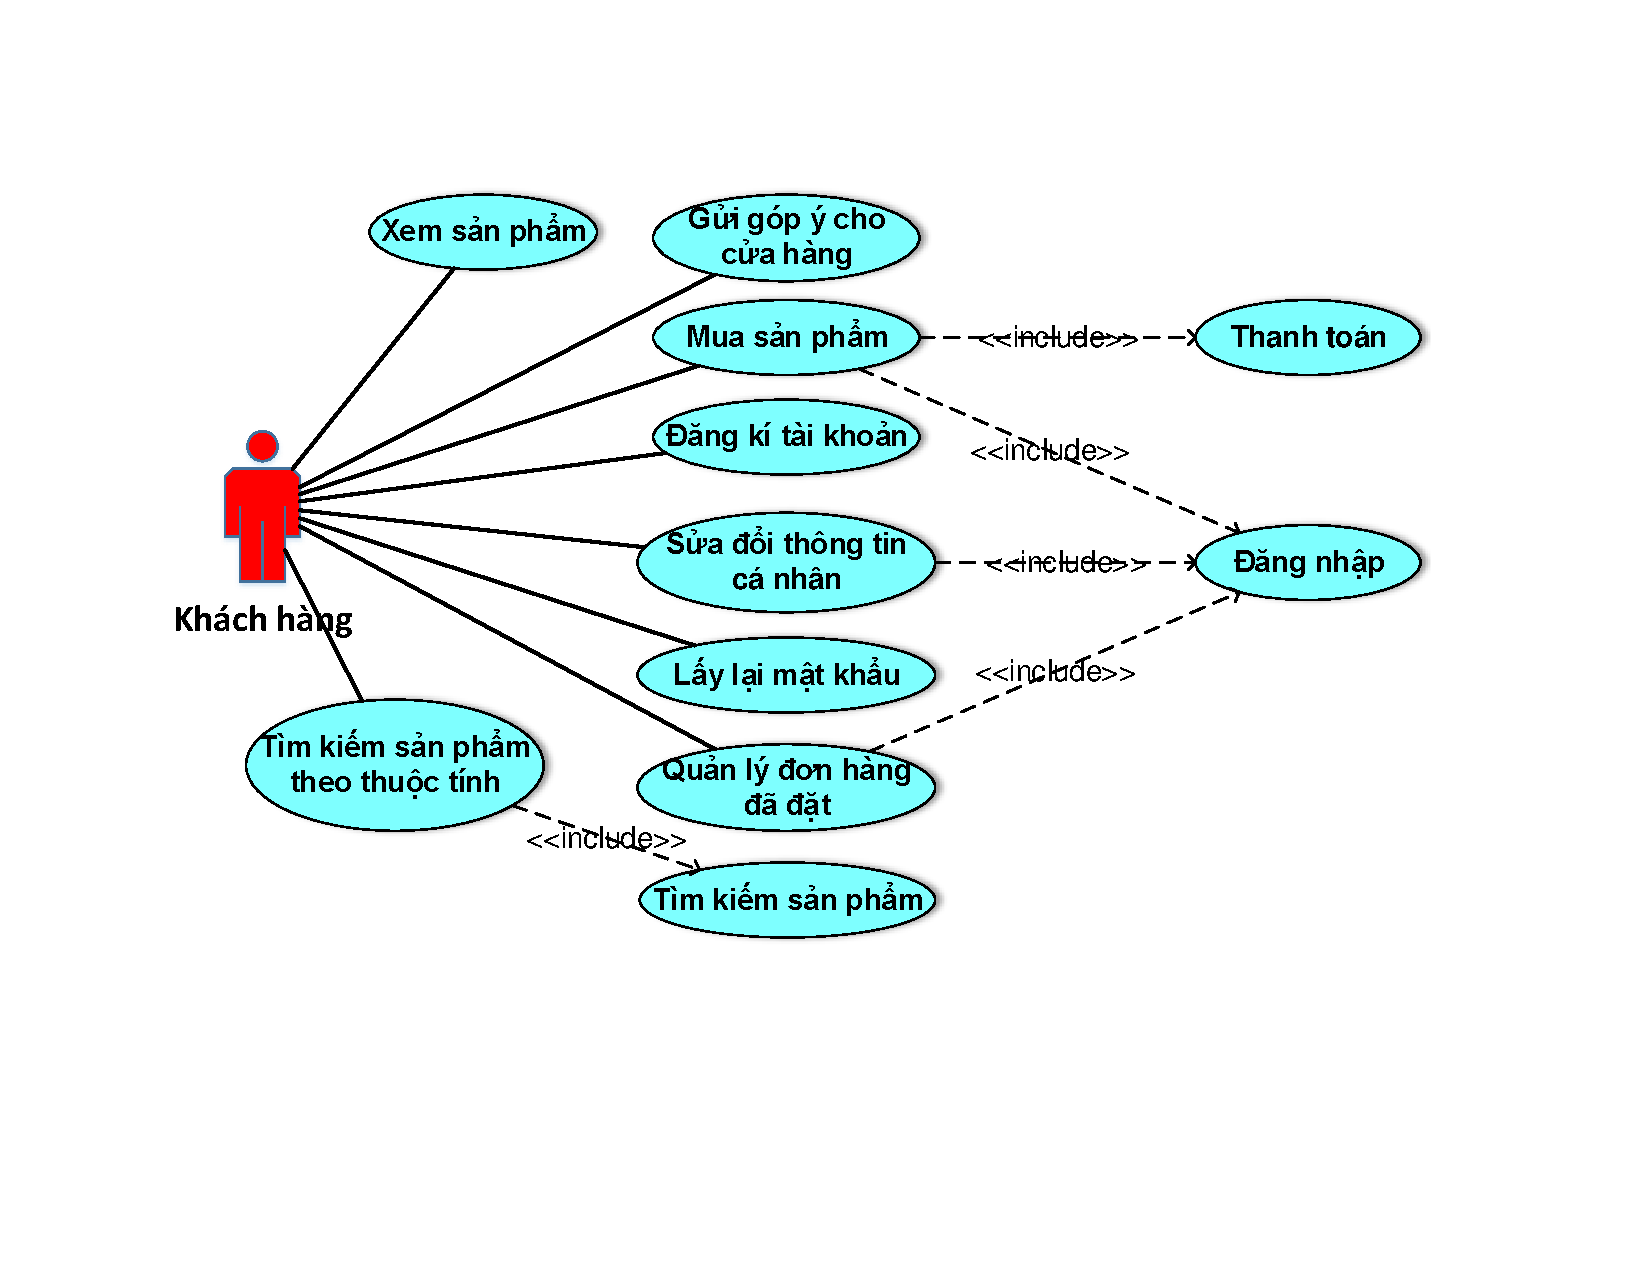
\includegraphics[scale=0.7]{image/UseCaseTongQuanKH.pdf}
    \end{center}
    \caption{Use-Case Khách hàng}
    \label{refhinh3_3}
    \end{figure}
\end{center}
Từ Hình \ref{refhinh3_3} ta có các bảng đặc tả chi tiết cho các Use-Case của khách hàng:
\par
- Use-Case đăng nhập:
\begin{longtable}[htp]{ |m{0.25\linewidth}|m{0.65\linewidth}|}
 \caption{Bảng Use-Case đăng nhập \label{long}}\\
 \hline
 Use-Case & Nội dung \\
 \hline
 Tên Use-Case & Đăng nhập \\
 \hline
 Mô tả & Use-case cho phép khách hàng đăng nhập vào trang chủ để thưc hiện việc mua bán theo như cầu khách hàng\\
 \hline
 Tên tác nhân & Khách hàng\\
 \hline
 Điều kiện kích hoạt & Khách hàng vào trang chủ và nhận nút đăng nhập\\
 \hline
 Tiền điều kiện & Khách hàng đã đăng ký tài khoản trên hệ thống\\
 \hline
 Hậu điều kiện & Khách hàng đăng nhập thành công\\
 \hline
 Luồng sự kiện chính & 
  1. Hệ thống hiện thị màn hình đăng nhập.\newline
  2. Khách hàng nhập tên đăng nhập và mật khẩu.\newline
  3. Hệ thống kiểm tra thông tin đăng nhập.\newline
  4. Nếu thành công hệ thống sẽ đưa khách hàng về trang chủ.\newline
  5. Kết thúc Use-case.	
 \\
 \hline
 Luồng sự kiện phụ & 
 - Tài khoản và mật khẩu không hợp lệ:\newline
 1. Khi khách hàng nhập sai tên đăng nhập và mật khẩu\newline
 2. Hệ thống hiển thị lại màn hình đăng nhập để khách hàng nhập lại thông tin tài khoản và mật khẩu kèm theo thông báo tên đăng nhập và mật khẩu bị sai.\newline
  Quay lại bước 2 trong luồng sự kiện chính.
 \\
 \hline
\end{longtable}
\par
- Use-Case tìm kiếm sản phẩm:
\begin{longtable}[htp]{ |m{0.25\linewidth}|m{0.65\linewidth}|}
 \caption{Bảng Use-Case tìm kiếm sản phẩm \label{long}}\\
 \hline
 Use-Case & Nội dung \\
 \hline
 Tên Use-Case & Tìm kiếm sản phẩm \\
 \hline
 Mô tả & Use-case cho phép khách hàng tìm kiếm các sản phẩm có trong hệ thống theo tên sản phẩm giúp cho khách hàng tiết kiệm thời gian nhất có thể.\\
 \hline
 Tên tác nhân & Khách hàng\\
 \hline
 Điều kiện kích hoạt & Khách hàng truy cập vào trang chủ và nhập dữ liệu cần tìm vào ô tìm kiếm\\
 \hline
 Tiền điều kiện & Khách hàng truy cập vào trang chủ\\
 \hline
 Hậu điều kiện & Tìm kiếm được kết quả về sản phẩm\\
 \hline
 Luồng sự kiện chính & 
  1. Hệ thống hiện thị ô tìm kiếm và yêu cầu người dùng nhập dữ liệu cần tìm kiếm.\newline
  2. Khách hàng nhập dữ liệu cần tìm kiếm.\newline
  3. Hệ thống kiểm tra dữ liệu cần tìm kiếm và sẽ đưa ra gợi ý cho người dùng theo từng kí tự người dùng nhập vào.\newline
  4. Khách hàng lựa chọn 1 sản phẩm đúng theo ý khách hàng dựa trên các gợi ý mà hệ thống đã đưa ra\newline
  5. Kết thúc Use-case.	
 \\
 \hline
 Luồng sự kiện phụ & 
 - Sản phẩm không có trên hệ thống:\newline
 1. Hệ thống kiểm tra theo dữ liệu người dùng nhập vào, dữ liệu người dùng nhập vào không khớp với dữ liệu trong cơ sở dữ liệu hệ thống sẽ hiển thị thông báo không có sản phẩm.\newline
  Quay lại bước 2 trong luồng sự kiện chính.
 \\
 \hline
\end{longtable}

- Use-Case mua sản phẩm:
\begin{longtable}[htp]{ |m{0.25\linewidth}|m{0.65\linewidth}|}
 \caption{Bảng Use-Case mua sản phẩm \label{long}}\\
 \hline
 Use-Case & Nội dung \\
 \hline
 Tên Use-Case & Mua sản phẩm \\
 \hline
 Mô tả & Use-case cho phép khách hàng có thể đặt hàng ngay trên trang chủ.\\
 \hline
 Tên tác nhân & Khách hàng\\
 \hline
 Điều kiện kích hoạt & Khách hàng truy cập vào trang chủ và nhấn vào nút giỏ hàng để tiên hàng đặt hàng \\
 \hline
 Tiền điều kiện & Khách hàng truy cập vào trang chủ và đã đăng nhập vào trang chủ\\
 \hline
 Hậu điều kiện & Thông tin đơn hàng được lưu xuống cơ sở dữ liệu\\
 \hline
 Luồng sự kiện chính & 
  1. Hệ thống hiện thị giao diện đặt hàng và yêu cầu người dùng nhập thông tin đặt hàng.\newline
  2. Khách hàng nhập thông tin đặt hàng .\newline
  3. Hệ thống kiểm tra thông tin đơn hàng và xác nhận hợp lệ.\newline
  4. Hệ thống thông báo đã đặt hàng thành công và đưa khách hàng về trang đơn hàng của tài khoản đang được đăng nhập\newline
  5. Sẽ có điện thoại từ cửa hàng cho khách hàng để xác nhận đơn hàng.
  5. Kết thúc Use-case.	
 \\
 \hline
 Luồng sự kiện phụ & 
 - Khách hàng chưa đăng nhập:\newline
 1.Hệ thống yêu cầu khách hàng đăng nhập trước khi nhấn nút đặt hàng.\newline
  Quay lại bước 1 trong luồng sự kiện chính.
 \\
 \hline
\end{longtable}

-Use-Case thanh toán:
\begin{longtable}[htp]{ |m{0.25\linewidth}|m{0.65\linewidth}|}
 \caption{Bảng Use-Case thanh toán sản phẩm \label{long}}\\
 \hline
 Use-Case & Nội dung \\
 \hline
 Tên Use-Case & Thanh toán sản phẩm \\
 \hline
 Mô tả & Use-case cho phép khách hàng thanh toán trực tuyển các đơn hàng thông qua cổng thanh toán trực tuyển ngân lượng.\\
 \hline
 Tên tác nhân & Khách hàng\\
 \hline
 Điều kiện kích hoạt & Khách hàng truy cập vào trang chủ và nhấn vào nút thanh toán của ngân lượng có trên hoá đơn đặt hàng.\\
 \hline
 Tiền điều kiện & Khách hàng truy cập vào trang chủ đã đăng nhập và có tài khoản ngân lượng với số dự lớn hơn đơn hàng là 2\%.\\
 \hline
 Hậu điều kiện & Nhận được mail thanh toán thành công gửi từ ngân lượng và điện thoại xác nhận từ chủ cửa hàng.\\
 \hline
 Luồng sự kiện chính & 
  1. Khách hàng chọn hoá đơn cần thanh toán trong danh sách hoá đơn mà người dùng đã đặt.
  2. Khách hàng nhấn nút thanh toán để chuyển đến trang giao dịch của ngân lượng.\newline
  3. Khách hàng nhập thông tin tài khoản ngân lượng để tiến hàng giao dịch đơn hàng.\newline
  4. Hệ thông ngân lượng xác nhận lại thông tin đơn hàng.\newline
  5. Khách hàng chọn tiến hàng thanh toán để ngân lượng gửi mã OTP về số điện thoại mà khách hàng đã đăng ký.\newline
  6. Khách hàng nhập mã OTP.\newline 
  7. Hệ thống ngân lượng kiểm tra mã OTP và xác nhận thanh toán.\newline 
  8. Hệ thống ngân lượng sẽ gửi mail cho khách hàng và chủ cửa hàng về thông tin đơn hàng.\newline 
  9. Chủ cửa hàng sẽ xác nhận lại thông tin rồi gọi điện thoại cho khách hàng để chứng thực lại thông tin đơn hàng sau đó sẽ vận chuyển hàng cho khách hàng.\newline 
  5. Kết thúc Use-case.	\newline 
 \\
 \hline
 Luồng sự kiện phụ & 
 - Khách hàng nhập sai tài khoản ngân lượng:\newline
 1. Khi khách hàng nhập sai tên đăng nhập và mật khẩu.\newline
 2. Hệ thống ngân lượng sẽ hiển thị lại màn hình đăng nhập đồng thời hiển thị thông báo đăng nhập không thành công 
  Quay lại bước 3 trong luồng sự kiện chính.
 \\
 \hline
\end{longtable}
\newpage
\subsubsection{Nhân viên quản lý}
\begin{center}
    \begin{figure}[h]
    \begin{center}
     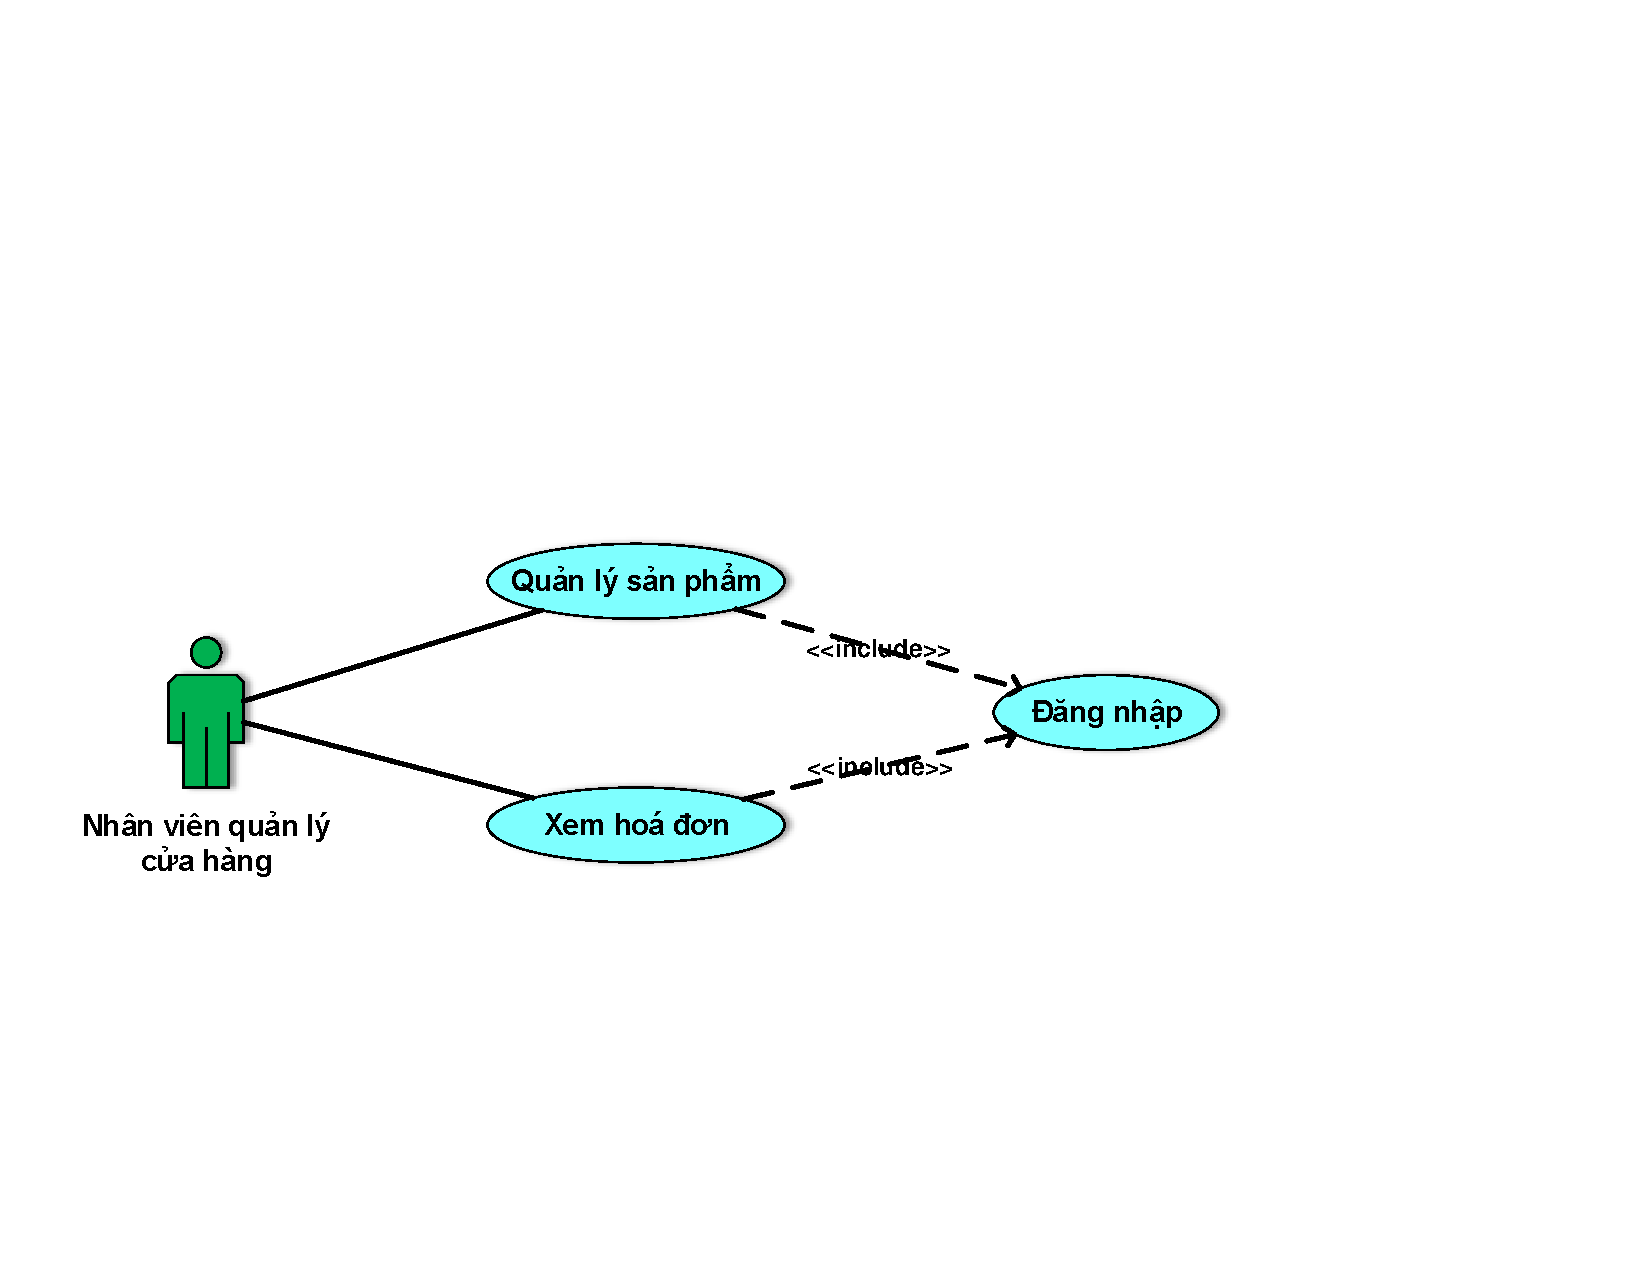
\includegraphics[scale=0.7]{image/UseCaseTongQuanNV.pdf}
    \end{center}
    \caption{Use-Case Nhân viên quản lý}
    \label{refhinh3_4}
    \end{figure}
\end{center}
Hình \ref{refhinh3_4} là use case tổng quan của nhân viên quản lý, nhân viên quản lý trong hệ thống chỉ được phép thêm và xem sản phẩm cũng như xem hoá đơn để xác nhận đơn hàng giúp chủ cửa hàng. Đặc tả chi tiết của use case nhân viên quản lý được thể hiện ở các bảng sau:
\begin{itemize}
\item Đăng nhập được thể hiện ở Bảng \ref{login}
\item Đăng xuất được thể hiện ở Bảng \ref{logout}
\item Thêm sản phẩm được thể hiện ở Bảng \ref{createProduct}
\item Sửa sản phẩm được thể hiện ở Bảng \ref{updateProduct}
\item Xem hoá đơn sản phẩm được thể hiện ở Bảng \ref{listBill}
\end{itemize}
\subsubsection{Người vận chuyển}
\begin{center}
    \begin{figure}[h]
    \begin{center}
     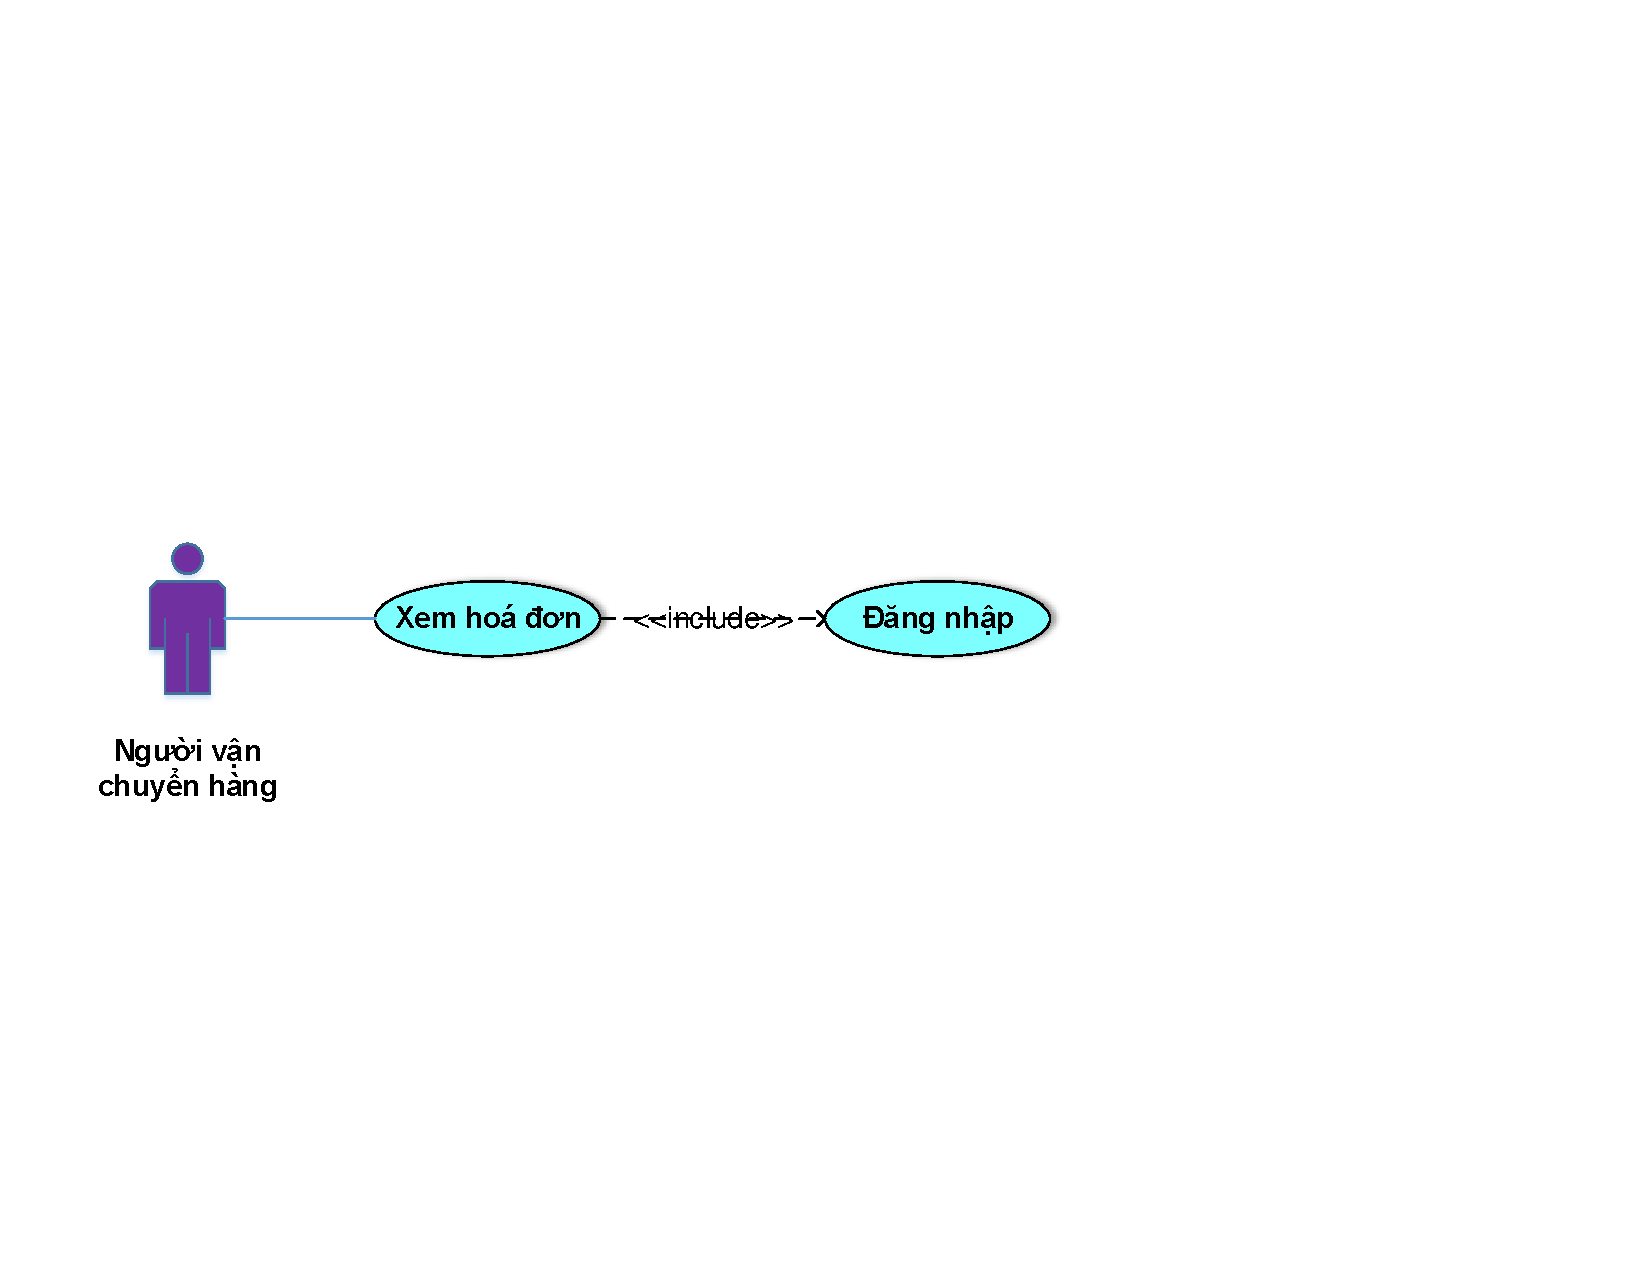
\includegraphics[scale=0.7]{image/UseCaseTongQuanNVC.pdf}
    \end{center}
    \caption{Use-Case Người vận chuyển}
    \label{refhinh3_5}
    \end{figure}
\end{center}
Hình \ref{refhinh3_5} là use case tổng quan của người vận chuyển, người vận chuyển trong hệ thống chỉ được phép xem hoá đơn để xme những đơn hàng nào cần giao hàng. Đặc tả chi tiết của use case người vận chuyển được thể hiện ở các bảng sau:
\begin{itemize}
\item Đăng nhập được thể hiện ở Bảng \ref{login}
\item Đăng xuất được thể hiện ở Bảng \ref{logout}
\item Xem hoá đơn sản phẩm được thể hiện ở Bảng \ref{listBill}
\end{itemize}
\subsection{Biểu đồ tuần tự(sequence diagram)}
Biểu đồ tuần tự minh họa các đối tượng tương tác với nhau ra sao. Chúng tập trung vào các chuỗi thông điệp, có nghĩa là các thông điệp được gửi và nhận giữa một loạt các đối tượng như thế nào. Biểu đồ tuần tự có hai trục: trục nằm dọc chỉ thời gian, trục nằm ngang chỉ ra một tập hợp các đối tượng. Một biểu đồ tuần tự cũng nêu bật sự tương tác trong một kịch bản – một sự tương tác sẽ xảy ra tại một thời điểm nào đó trong quá trình thực thi của hệ thống.
\begin{itemize}
\item Mục đích: biểu diễn tương tác giữa những người dùng và những đối tượng bên trong hệ thống. Biểu đồ này cho biết các thông điệp được truyền tuần tự như thế nào theo thời gian. Thứ tự các sự kiện trong biểu đồ tuần tự hoàn toàn tương tự như trong kịch bản mô tả use case tương ứng.
\item Biểu diễn: Biểu đồ tuần tự được biểu diễn bởi các đối tượng và thông báo truyền đi giữa các đối tượng đó. Trong hệ thống website thương mại điện tử, chúng ta lựa chọn biểu đồ tương tác dạng tuần tự để biểu diễn các tương tác giữa các đối tượng. Để xác định rõ các thành phần cần bổ sung trong biểu đồ lớp, trong mỗi biểu đồ tuần tự của hệ thống quản lý bán hàng sẽ thực hiện:
\begin{itemize}
\item Xác định rõ kiểu của đối tượng tham gia trong tương tác (ví dụ giao diện, điều khiển hay thực thể).
\item Mỗi biểu đồ tuần tự có thể có ít nhất một lớp giao diện tương ứng với chức năng (use case) mà biểu đồ đó mô tả.
\item Mỗi biểu đồ tuần tự có thể liên quan đến một hoặc nhiều đối tượng thực thể. Các đối tượng thực thể chính là các  đối tượng của các lớp  đã được xây dựng trong biểu đồ thiết kế chi tiết.
\end{itemize}
\end{itemize}
\par
Dưới đây là một số biểu đồ tuần tự cho các chức năng của hệ thống quản lý bán hàng:





\chapter{Triển khai, kiểm thử và kết quả}
\label{chapter4}
Sau khi đã phân tích các chức năng và nghiệp vụ của từng đối tượng trong hệ thống cũng như xây dựng được cơ sở dữ liệu hoàn chỉnh, em sẽ tiến hành triển khai hệ thống theo các chức năng đã được nêu ra ở Chương \ref{chapter3} cùng với đó em sẽ đưa ra một số trường hợp để kiểm thử các chức năng và hướng phát triển của đề tài.
\section{Triển khai hệ thống}
Để triển khai hệ thống em dùng một số Design Pattern:
\begin{itemize}
\item Repository là một pattern để tạo ra một lớp interface trung gian giữa lớp data và lớp business. Lớp này chứa đựng phương thức thao tác mà để giao tiếp với lớp dữ liệu và phục vụ cho nghiệp vụ từ lớp logic . Mục đích tạo ra lớp này để cách ly với việc tiếp cận dữ liệu sao cho những thay đổi không ảnh hưởng trực tiếp đến lớp logic nghiệp vụ.
\item Dependency Injection là một pattern rất phổ biến hiện nay nó giảm sự phụ thuộc của module cấp cao vào module cấp thấp mà cả hai module cùng phụ thuộc vào một interface. Các lớp giao tiếp với nhau thông qua interface mà không thông qua các lớp triển khai.
\item Unit Of Work được sử dụng để đảm bảo nhiều hành động như insert, update, delete...được thực thi trong cùng một interface thống nhất, nghĩa là khi một hành động của người dùng tác động vào hệ thống, tất cả các hành động như insert, update, delete...phải thực hiện xong thì mới gọi là một transaction thành công. Gói tất cả các hành động đơn lẻ vào một transaction để đảm bảo tính toàn vẹn dữ liệu.	
\end{itemize}
\begin{center}
    \begin{figure}[h]
    \begin{center}
     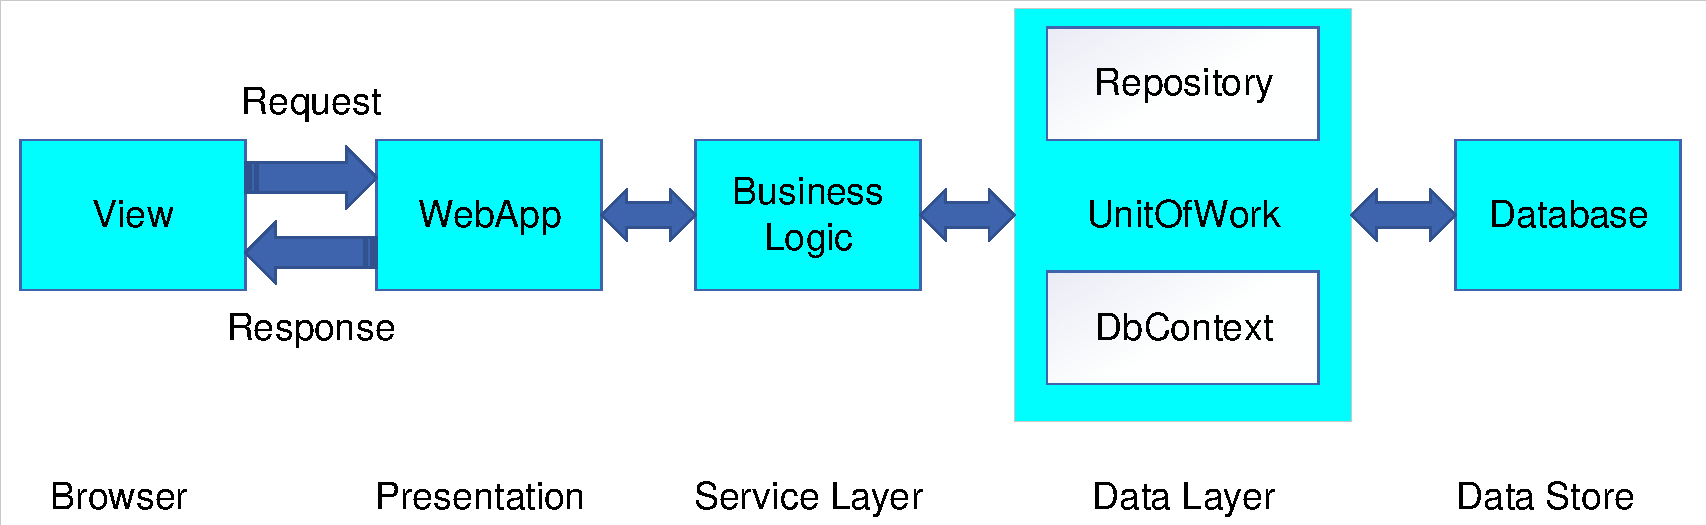
\includegraphics[scale=0.6]{image/MohinhDuongDiDuLieu.pdf}
    \end{center}
    \caption{Mô hình triển khai hệ thống}
    \label{refhinh4_1}
    \end{figure}
\end{center}

\par
Hình \ref{refhinh4_1} là mô hình tổng quan triển khai hệ thống bao gồm các tầng sau:
\begin{itemize}
\item Tầng View: tầng hiển thị giao diện cho người dùng.
\item Tầng WebApp: tầng tiếp nhận yêu cầu của người dùng để xử lý và trả dữ liệu đến view hiển thị lên giao diện người dùng, đây cũng là tầng trung gian giữa giao diện và dữ liệu nói cách khác WebApp là tầng điều khiển dữ liệu cho hệ thống.
\item Tầng Business Logic: tầng này xử lý các nghiệp vụ của từng thực thể có trong hệ thống như là sản phẩm, tài khoản, đơn hàng,...
\item Tầng Data Layer: tầng này đảm nhận việc điều khiển dữ liệu trong cơ sở dữ liệu thông qua Entity Framework, nó giúp hệ thống gọi đến cơ sở dữ liệu và thực hiện lấy đúng dữ liệu theo yêu cầu của người dùng.
\item Tầng Data Store: tầng này có nhiệm vụ lưu trữ dữ liệu cho hệ thống.
\end{itemize}
\par
Từ Hình \ref{refhinh4_1} em chia hệ thống thành 5 project theo như phân tầng đã trình bày ở trên. Đặt tên project của hệ thống là ShoppingOnline và mỗi project nhỏ sẽ được đặt tên theo quy tắc ShoppingOnline cộng với tên project nhỏ:
\begin{itemize}
\item ShoppingOnline.Infrastructure: Project này để hạng tầng chung của hệ thống.
\item ShoppingOnline.Utilities: Project này để khai báo các lớp tiện ích như: các hằng số, một số lớp mở rộng.
\item ShoppingOnline.Data: Project này để khai báo các thực thể có trong cơ sở dữ liệu.
\item ShoppingOnline.Data.EF: Project này gồm có: triển khai các repository, chứa DbContext  để thực hiện các truy vấn và kết nối đến cơ sở dữ liệu.
\item ShoppingOnline.Application: Project này triển khai các chức năng của mỗi thực thể có trong hệ thống.
\item ShoppignOnline.Application.Dapper: Project bao gồm một số chức năng mà Entity Framework không hỗ trợ nên phải dùng ngôn ngữ SQL thuần để truy vấn dữ liệu.
\item ShoppingOnline.WebApplication: Project được chạy lên đầu tiên khi bắt đầu hệ thống nó gồm có Controller để điểu khiển qua lại các yêu cầu từ View, một số tệp dùng để cài đặt Dependency Injection và cài đặt một số framework sử dụng thêm. 
\end{itemize}

\section{Kiểm thử hệ thống và kết quả}
\subsection{Kiểm thử}
- Kiểm thử chức năng đăng nhập:
\begin{longtable}[htp]{ |m{0.2\linewidth}|m{0.2\linewidth}|m{0.2\linewidth}|m{0.2\linewidth}|m{0.1\linewidth}|}
 \caption{Bảng kiểm thử chức năng đăng nhập \label{updateProduct}}\\
 \hline
Bước kiểm tra & Dữ liệu nhập vào & Kết quả dự kiến & Kết quả thực tế & Trạng thái \\
 \hline
Điều hướng đúng đến trang đăng nhập quản trị & &Người dùng đến được trang đăng nhập quản trị & Như dự kiến & Thành công\\
 \hline
 Nhập tên tài khoản & admin & Nhập được dữ liệu trên màn hình & Như dự kiến & Thành công\\
 \hline
  Nhập mật khẩu & 123654\$ & Nhập được dữ liệu trên màn hình & Như dự kiến & Thành công\\
 \hline
  Nhấn vào nút đăng nhập & & Người dùng được đăng nhập vào trang chủ quản trị & Như dự kiến & Thành công\\
 \hline
  Chuyển đến trang chủ quản trị & & Màn hình hiển thị thanh menu chức năng theo đúng quyền mà tài khoản được cấp & Như dự kiến & Thành công\\
 \hline
\end{longtable}

- Kiểm thử chức năng đăng xuất:
\begin{longtable}[htp]{ |m{0.2\linewidth}|m{0.2\linewidth}|m{0.2\linewidth}|m{0.2\linewidth}|m{0.1\linewidth}|}
 \caption{Bảng kiểm thử chức năng đăng xuất \label{updateProduct}}\\
 \hline
 Bước kiểm tra & Dữ liệu nhập vào & Kết quả dự kiến & Kết quả thực tế & Trạng thái \\
 \hline
  Nhấn vào nút đăng xuất & & Người dùng được chuyển về trang đăng xuất & Như dự kiến & Thành công\\
 \hline
\end{longtable}

- Kiểm thử chức năng quản lý tài khoản người dùng:
\begin{longtable}[htp]{ |m{0.2\linewidth}|m{0.2\linewidth}|m{0.2\linewidth}|m{0.2\linewidth}|m{0.1\linewidth}|}
 \caption{Bảng kiểm thử chức năng thêm tài khoản người dùng \label{updateProduct}}\\
 \hline
 Bước kiểm tra & Dữ liệu nhập vào & Kết quả dự kiến & Kết quả thực tế & Trạng thái \\
 \hline
  Nhấn vào nút thêm tài khoản người dùng & & Giao diện hiển thị modal nhập thông tin tài khoản & Như dự kiến & Thành công\\
 \hline
   Nhập tên đầy đủ & Lê Bá Tuấn Anh & Nhập được dữ liệu trên màn hình & Như dự kiến & Thành công\\
 \hline
   Nhập tên tài khoản & lebatuananh & Nhập được dữ liệu trên màn hình & Như dự kiến & Thành công\\
 \hline
   Nhập ngày sinh & 30/04/1996 & Nhập được dữ liệu trên màn hình & Như dự kiến & Thành công\\
 \hline
   Nhập mật khẩu & 123654 & Nhập được dữ liệu trên màn hình & Như dự kiến & Thành công\\
 \hline
   Nhập lại mật khẩu & 123654 & Nhập được dữ liệu trên màn hình & Như dự kiến & Thành công\\
 \hline
   Nhập email & tuananh300496 @gmail.com & Nhập được dữ liệu trên màn hình & Như dự kiến & Thành công\\
 \hline
   Nhập địa chỉ & Hà Nội & Nhập được dữ liệu trên màn hình & Như dự kiến & Thành công\\
 \hline
   Nhập số điện thoại & 0333355553 & Nhập được dữ liệu trên màn hình & Như dự kiến & Thành công\\
 \hline
   Chọn giới tính & Male & Nhập được dữ liệu trên màn hình & Như dự kiến & Thành công\\
 \hline
   Chọn nhóm quyền cho tài khoản & Top Manager & Nhập được dữ liệu trên màn hình & Như dự kiến & Thành công\\
 \hline
    Chọn trạng thái tài khoản & Active & Nhập được dữ liệu trên màn hình & Như dự kiến & Thành công\\
 \hline
    Nhấn nút lưu tài khoản && Hiển thị thông báo tài khoản được lưu và chuyển về trang danh sách tài khoản  & Như dự kiến & Thành công\\
 \hline
\end{longtable}

- Kiểm thử chức năng quản lý sản phẩm:
\begin{longtable}[htp]{ |m{0.2\linewidth}|m{0.2\linewidth}|m{0.2\linewidth}|m{0.2\linewidth}|m{0.1\linewidth}|}
 \caption{Bảng kiểm thử chức năng thêm sản phẩm \label{updateProduct}}\\
 \hline
 Bước kiểm tra & Dữ liệu nhập vào & Kết quả dự kiến & Kết quả thực tế & Trạng thái \\
 \hline
  Nhấn vào nút thêm sản phẩm & & Giao diện hiển thị modal nhập thông tin sản phẩm & Như dự kiến & Thành công\\
 \hline
   Nhập tên sản phẩm & Sản phẩm Test & Nhập được dữ liệu trên màn hình & Như dự kiến & Thành công\\
 \hline
   Chọn danh mục sản phẩm & Women shirt & Nhập được dữ liệu trên màn hình & Như dự kiến & Thành công\\
 \hline
   Nhập mô tả cho sản phẩm & Sản phẩm Test & Nhập được dữ liệu trên màn hình & Như dự kiến & Thành công\\
 \hline
   Nhập đơn vị & chiếc & Nhập được dữ liệu trên màn hình & Như dự kiến & Thành công\\
 \hline
   Nhập giá bán  & 10000 & Nhập được dữ liệu trên màn hình & Như dự kiến & Thành công\\
 \hline
   Nhập giá nhập & 5000 & Nhập được dữ liệu trên màn hình & Như dự kiến & Thành công\\
 \hline
   Nhập giá khuyến mại & 8000 & Nhập được dữ liệu trên màn hình & Như dự kiến & Thành công\\
 \hline
   Tải ảnh lên và chọn kích cỡ cho ảnh & 0333355553 & Tải được dữ liệu trên màn hình & Như dự kiến & Thành công\\
 \hline
   Soạn thảo nội dung cho sản phẩm & Sản phẩm Test & Nhập được dữ liệu trên màn hình & Như dự kiến & Thành công\\
 \hline
    Chọn trạng thái, sản phẩm hot, hiển thị trên trang chỉ sản phẩm & Active, Hot product, Show on home & Nhập được dữ liệu trên màn hình & Như dự kiến & Thành công\\
 \hline
    Nhấn nút lưu sản phẩm && Hiển thị thông báo sản phẩm được lưu và chuyển về trang danh sách sản phẩm  & Như dự kiến & Thành công\\
 \hline
\end{longtable}

\subsection{Kết quả}
Trên đây em trình bày kiểm thử một số chức năng chính của hệ thống vì trong lúc triển khai hệ thống em đã kiểm thử hết các chức năng của hệ thống và dưới đây là một số kết quả sau khi kiểm thử phần mềm.
 \begin{center}
    \begin{figure}[h]
    \begin{center}
     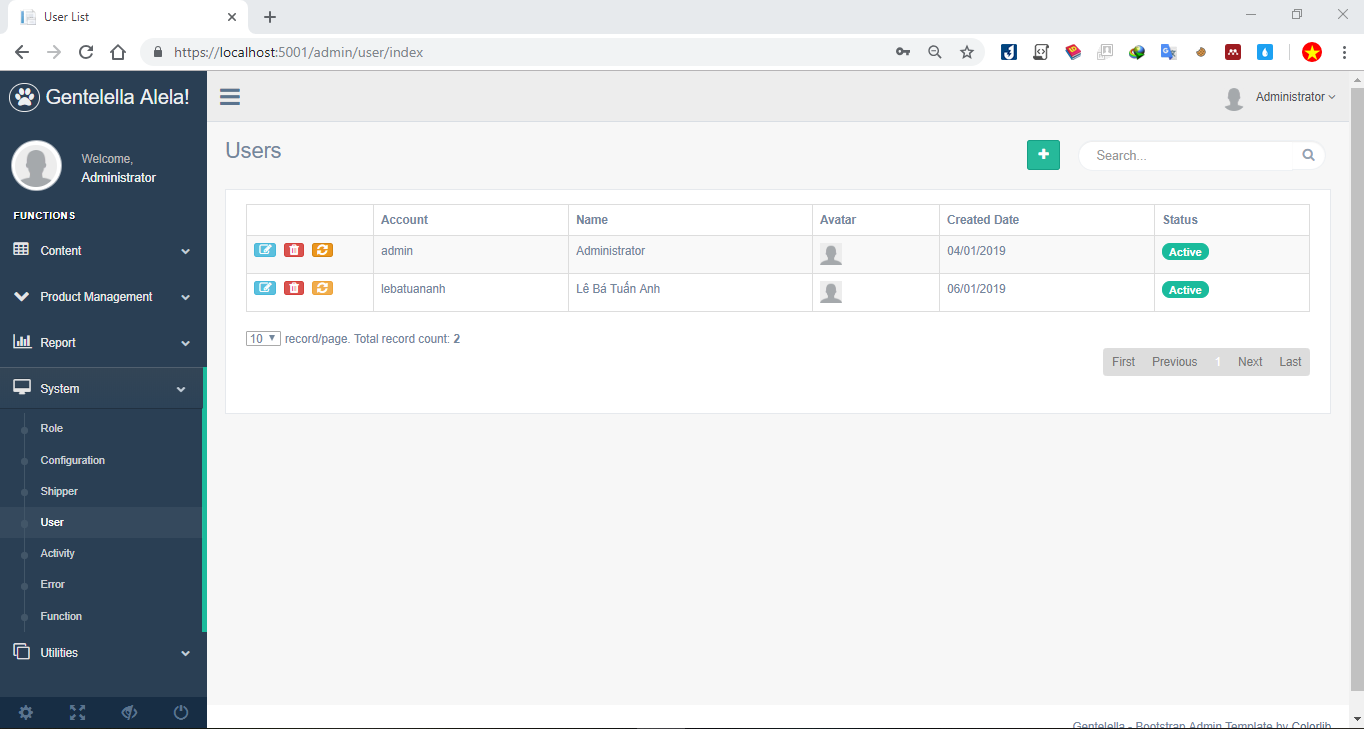
\includegraphics[scale=0.45]{image/danhsachTK}
    \end{center}
    \caption{Giao diện danh sách tài khoản}
    \label{refhinh4_2}
    \end{figure}
\end{center}
\par
Hình \ref{refhinh4_2} là màn hình sau khi kiểm thử chức năng thêm tài khoản người dùng. Một số hình dưới đây đều là kết quả thu được sau khi quá trình kiểm thử triển khai hệ thống, vì có nhiều chức năng nên em chỉ đưa ra những hình ảnh của chức năng nổi bật nhất.
 \begin{center}
    \begin{figure}[h]
    \begin{center}
     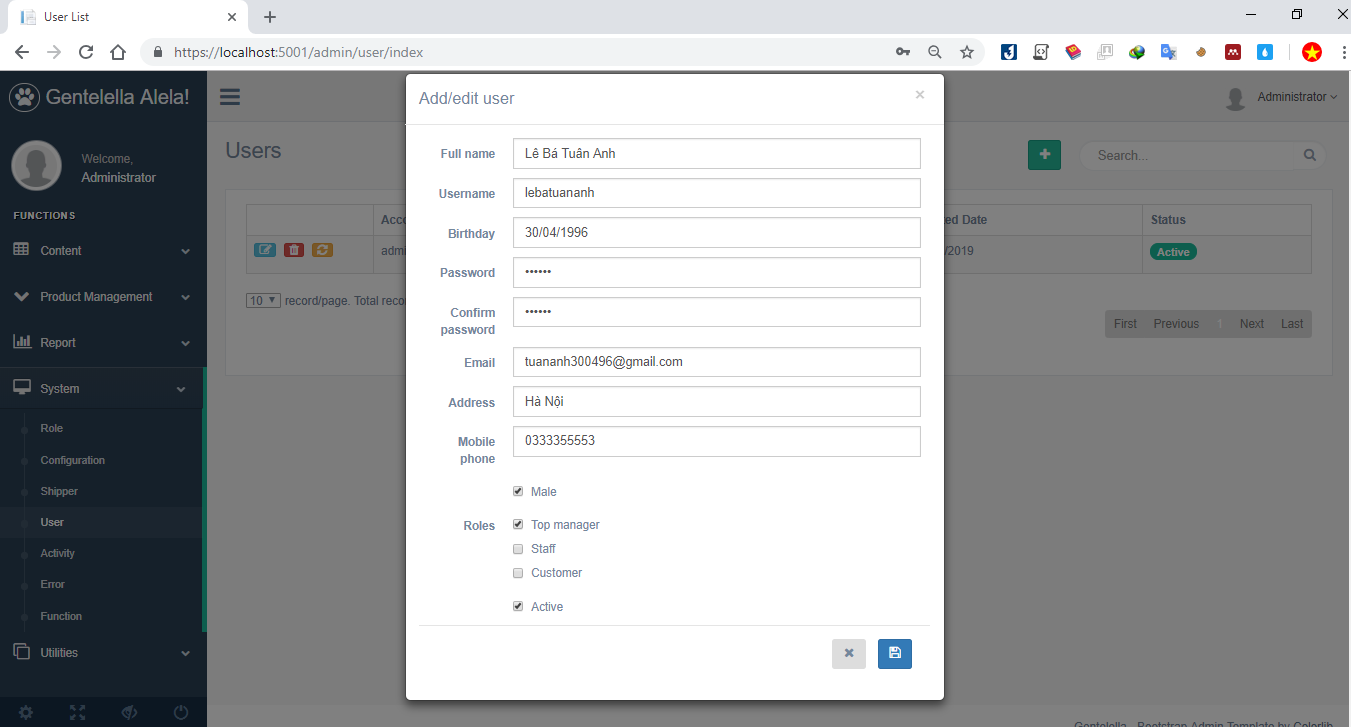
\includegraphics[scale=0.45]{image/themTK}
    \end{center}
    \caption{Giao diện thêm tài khoản}
    \label{refhinh4_3}
    \end{figure}
\end{center}

 \begin{center}
    \begin{figure}[h]
    \begin{center}
     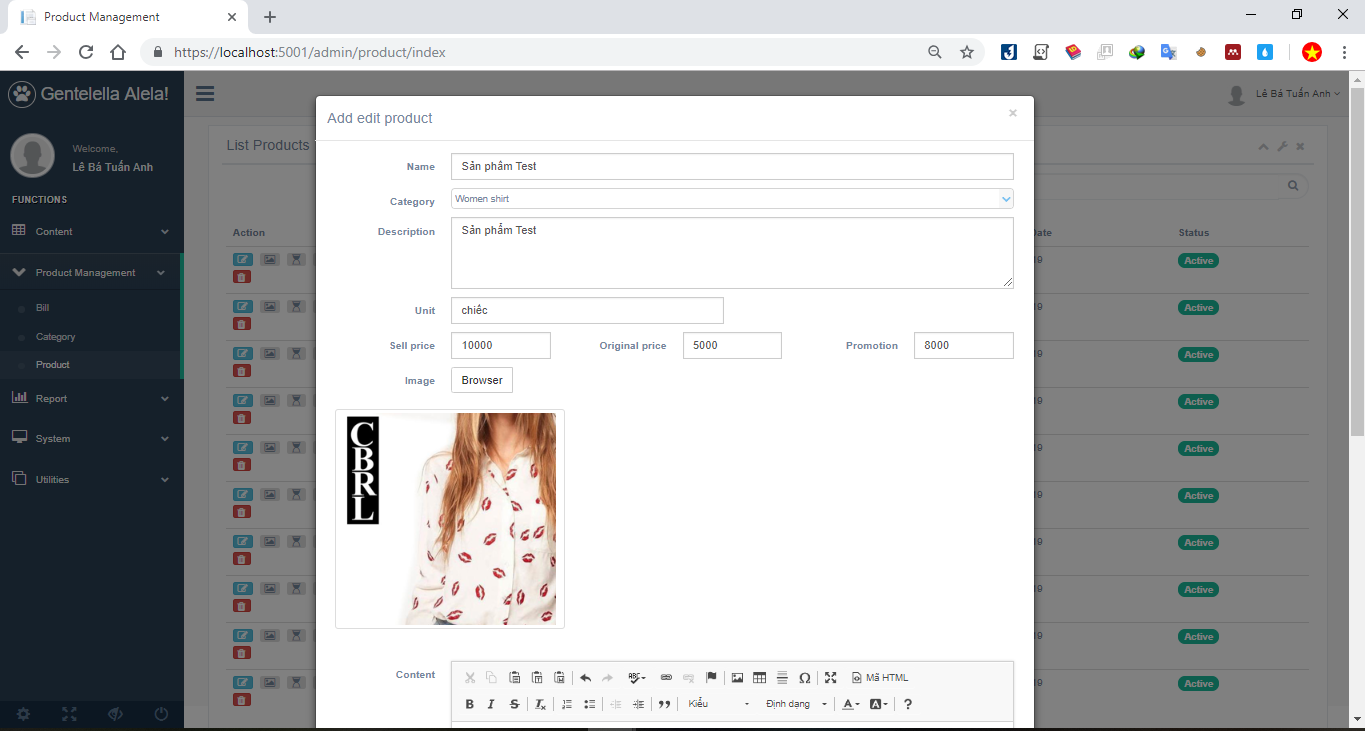
\includegraphics[scale=0.45]{image/themSanpham}
    \end{center}
    \caption{Giao diện thêm sản phẩm}
    \label{refhinh4_4}
    \end{figure}
\end{center}

\begin{center}
    \begin{figure}[h]
    \begin{center}
     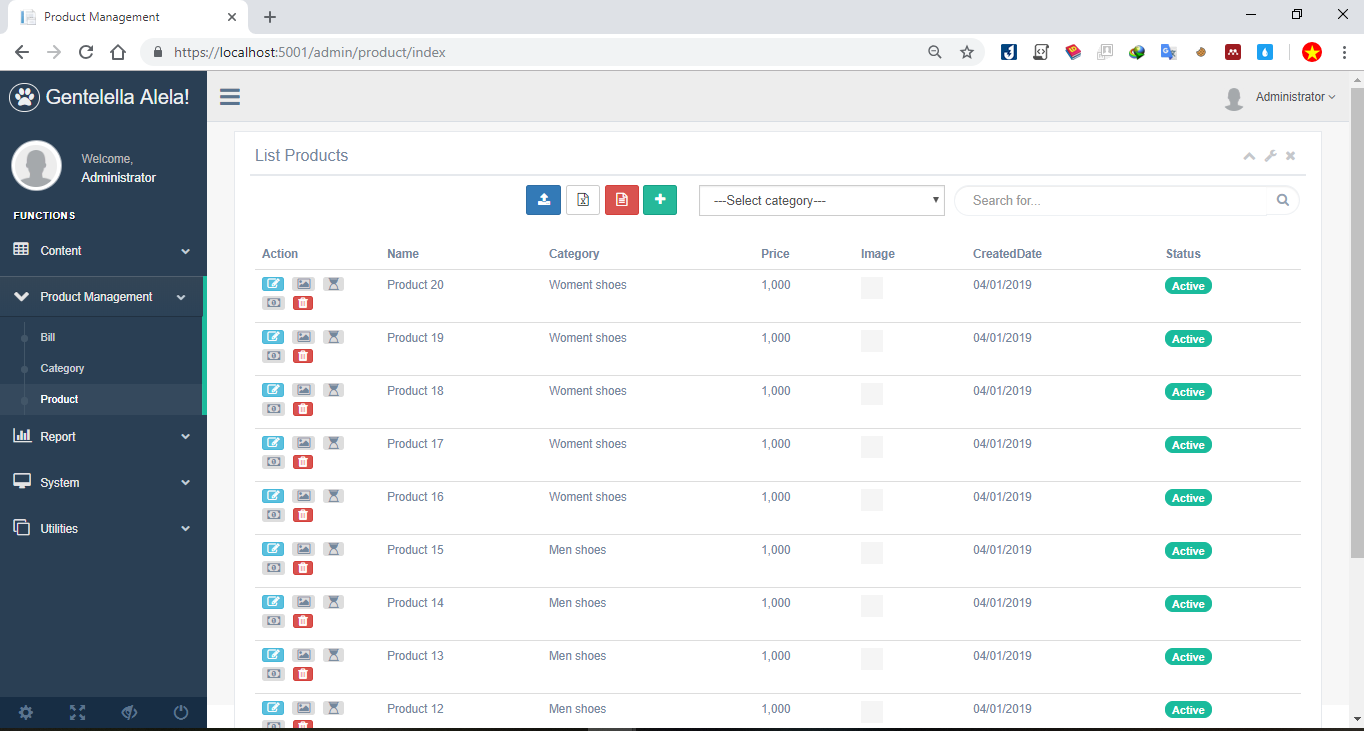
\includegraphics[scale=0.45]{image/danhsachSP}
    \end{center}
    \caption{Giao diện danh sách sản phẩm}
    \label{refhinh4_5}
    \end{figure}
\end{center}

\begin{center}
    \begin{figure}[h]
    \begin{center}
     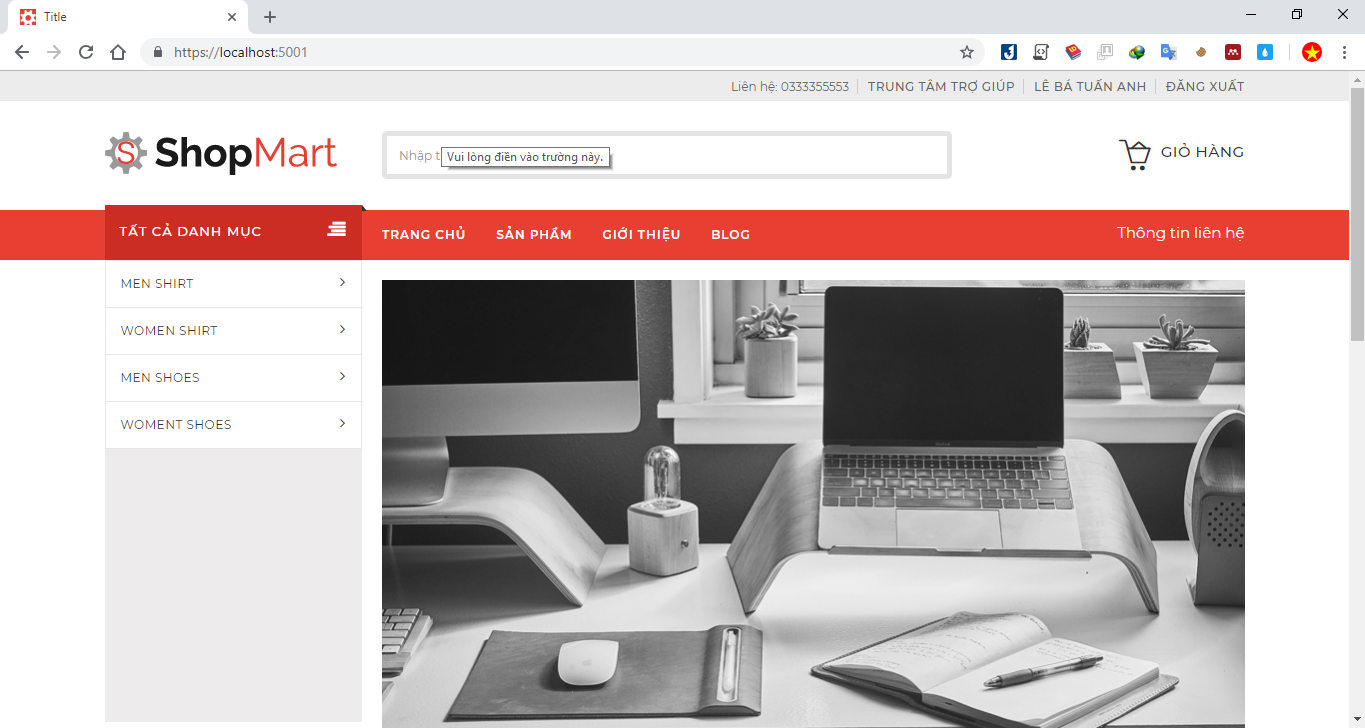
\includegraphics[scale=0.45]{image/trangchu}
    \end{center}
    \caption{Giao diện trang chủ}
    \label{refhinh4_6}
    \end{figure}
\end{center}






\thispagestyle{plain}
\chapter*{Kết luận}
\addcontentsline{toc}{chapter}{Kết luận}
Sau một thời gian làm đồ án, em nhận thấy bản thân đã có sự tiến bộ về khả nâng lập trình ứng dụng website, cải thiện tư duy về các sơ đồ chức năng mà nó gán liên với các thuật toán, khả năng đọc tài liệu trên internet cũng như cách tìm từ khoá trên Google để giải quyết vấn đề, nắm rõ được các công nghệ sử dụng có trong hệ thống. Việc thực hiện đồ án cũng giúp em có một sản phẩm để đi tuyển dụng đồng thời làm em hứng thú hơn với nghề lập trình viên. Sau đây em xin trình bày một số yêu cầu đã thực hiện được cùng với phương hướng phát triền đề tài
\par
- Hoàn thành hệ thống website thương mại điện tử với các chức năng:
\begin{itemize}
	\item Người quản trị quản lý sản phẩm, danh mục sản phẩm, hoá đơn bán hàng, doanh thu bán hàng, nhóm quyền, tài khoản người dùng, các thông tin liên quan đến trang web: quảng cáo, slide ảnh, thông tin cửa hàng,...
	\item Người dùng xem sản phẩm dễ dàng với chức năng tìm kiểm theo gợi ý, và theo sắp xếp các thuộc tính sản phẩm. Họ cũng có thể đặt hàng trên trang chủ cùng với đấy họ có thể thanh toán trực tuyền thông qua Ngân Lượng 
\end{itemize}

- Hướng phát triền của đề tài:
\begin{itemize}
\item Chỉnh sửa giao diện người dùng bắt mắt.
\item Phát triền việc dùng cơ sở dữ liệu bằng điện toán đám mây để tăng tốc độ tải dữ liệu.
\item Tối ưu hoá tốc độ truy vấn dữ liệu bằng ngôn ngữ NoSQL.
\end{itemize}
\par 
Trong quá trình nghiên cứu, xây dựng và thiết kế sản phẩm, em đã vấp phải nhiều khó khăn. Nhưng nhờ có sự hướng dẫn tận tình của TS. Trần Quang Vinh cũng như sự giúp đỡ của các thành viên trong phòng nghiên cứu Sanslab đã giúp em hoàn thiện đồ án này. Qua đó, giúp em củng cố thêm những kiến thức về website, lập trình; những kỹ năng làm việc nhóm, tìm hiểu nghiên cứu những vấn đề mới; cũng như có được những kiến thức mới và trải nghiệm thực tế.
\thispagestyle{plain}
\addcontentsline{toc}{chapter}{Tài liệu tham khảo}
\begin{thebibliography}{20}

\bibitem{1}
“11 trang web thương mại điện tử hàng đầu Việt Nam 2017.” [Online]. Available: https://giaidieu.com/blog/11-trang-web-thuong-mai-dien-tu-hang-dau-viet-nam-2017. [Accessed: 25-Dec-2018].

\bibitem{2}
“Introduction - The complete C\# tutorial.” [Online]. Available: https://csharp.net-tutorials.com/getting-started/introduction/. [Accessed: 25-Dec-2018].
\bibitem{3}
“jQuery API Documentation.” [Online]. Available: https://api.jquery.com/. [Accessed: 25-Dec-2018].
\bibitem{4}
“NET Framework Architecture Mono.” [Online]. Available: https://www.mono-project.com/archived/net-framework-architecture/. [Accessed: 25-Dec-2018].
\bibitem{5}
U. Noreen, A. Bounceur và L. Clavier, "A Study of LoRa Low Power and Wide Area Network Technology", 3${rd}$ International Conference on Advanced Technologies for Signal and Image Processing - ATSIP, Fez, Morroco, May 22-24, 2017.
\bibitem{6}
Andrew S. Tanenbaum, David J. Wetherall, \textit{"Computer Network"}, Prentice Hall, 2010.
\bibitem{7}
Module LoRa Ra-02 SX1278 datasheet (https://www.en.ai-thinker.com).
\bibitem{8}
SX1276/77/78 datasheet (https://www.semtech.com).
\bibitem{9}
STM32F1xC, STM32F1xD, STM32F1xE datasheet (https://www.st.com).
\bibitem{10}
STM32Cube initialization code generator.
\end{thebibliography}
\thispagestyle{plain}
\chapter*{Phụ lục}
\addcontentsline{toc}{chapter}{Phụ Lục}
\changefontsizes{11pt}
%\begin{mybox}
\begin{center}
\changefontsizes{13pt}{\textbf{Hàm main của Gateway}}
\end{center}
\begin{lstlisting}
int main(void)
{
  /* Reset of all peripherals, Initializes the Flash interface and the Systick. */
  HAL_Init();
  /* Configure the system clock */
  SystemClock_Config();
  /* Initialize all configured peripherals */
  MX_GPIO_Init();
  MX_DMA_Init();
  MX_SPI3_Init();
  MX_USART1_UART_Init();
  /* USER CODE BEGIN 2 */
  SX1278_Config();
  /* USER CODE END 2 */
  while (1)
  {
	uint8_t e = receivePacketTimeoutACK (&hspi3, 10000);
	if (!e){
		UART_print ("\nReceive msg");
		char msg[40] = {0};
		for (uint8_t i = 0; i < packet_received.length; i++){
			msg[i] = (char)packet_received.data[i];
		}
		int ID = packet_received.src;
		if (msg[1] == 'D'){
			char title[100];
			sprintf(title, "\nReceive Data form node %d: ", ID);
			UART_print(title);
			UART_print(msg);
		}
		else checkNode(ID, msg);	
	}
	else UART_print ("\nDon't have msg");
  }
}
\end{lstlisting}
\newpage
\begin{center}
\changefontsizes{13pt}{\textbf{Hàm kiểm tra bản tin xác thực của Gateway}}
\end{center}
\begin{lstlisting}
void checkNode (int nodeAddr, char msg[]){
		char title[100];
		sprintf(title, "\nSend accepted Msg to Node %d", nodeAddr);
		char *response;
		uint8_t e;
		UART_print(title);
		if (msg[2] == 's' && msg[3] == 'a' && msg[4] == 'n' && msg[5] == 's' && msg[6] == 'l' && msg[7] == 'a' && msg[8] == 'b'){
			response = "1";
			UART_print ("\nGateway: 1");
			arrNodeAddr[numberofNode++] = nodeAddr;
		}
		else{
			response = "0";
			UART_print ("\nGateway: 0");
		}
		uint8_t cnt;
		do{ 
			e = sendPacketTimeoutACKRetries(&hspi3, nodeAddr, response);
			cnt++;
			HAL_Delay (5);
		}
		while (e > 0 && cnt < 3);
}
\end{lstlisting}
\newpage
\begin{center}
\changefontsizes{13pt}{\textbf{Hàm main của nút}}
\end{center}
\begin{lstlisting}
int main(void)
{
  /* MCU Configuration----------------------------------------------------------*/
  /* Reset of all peripherals, Initializes the Flash interface and the Systick. */
  HAL_Init();
  /* Configure the system clock */
  SystemClock_Config();
  /* Initialize all configured peripherals */
  MX_GPIO_Init();
  MX_DMA_Init();
  MX_SPI3_Init();
  MX_USART1_UART_Init();
  /* USER CODE BEGIN 2 */
  SX1278_Config();
  /* USER CODE END 2 */
	delay = NODE_ADDRESS * 10;
	requestJoinNetwork(GWAY_ADDRESS);
  while (1)
  {
  /* USER CODE END WHILE */
		if (joinedNetwork == 1)
				sendData(GWAY_ADDRESS);
		HAL_Delay(15000);
  /* USER CODE BEGIN 3 */
  }
}
\end{lstlisting}
\newpage
\begin{center}
\changefontsizes{13pt}{\textbf{Hàm yêu cầu tham gia mạng của nút}}
\end{center}
\begin{lstlisting}
void requestJoinNetwork (uint8_t GWaddr)
{
		char msgRQ[20] = "@Rsanslab";
		uint8_t e;
		do{
				e	= sendPacketTimeoutACK (&hspi3, GWaddr , msgRQ);
				if (e == 0){
						UART_print ("\nSend msg_request successful, waiting msg_acception");
						uint8_t state = receivePacketTimeoutACK (&hspi3, 10000);
						char msgAccept[10] = {0};
						if (state == 0 && packet_received.src == GWAY_ADDRESS){
							for (uint8_t i = 0; i < packet_received.length; i++){
									msgAccept[i] = (char) packet_received.data[i];
							}
							if (msgAccept[0] == '1'){
									UART_print ("\nGateway accepted");
									joinedNetwork = 1;
							}
							else{
									UART_print ("\nGateway didn't accept");
									joinedNetwork = 2;
							}
							//delay = NODE_ADDRESS * 10;
						}
				}
				else{
					UART_print("\nSend msg_request nonsuccessful");
					//int x = rand() % 10;
					HAL_Delay (1000);
					//delay *= 2;
				}
		}
		while (e);
}
\end{lstlisting}
\newpage
\begin{center}
\changefontsizes{13pt}{\textbf{Hàm gửi dữ liệu của nút}}
\end{center}
\begin{lstlisting}
void sendData (uint8_t GWAddr){
		char msgData[100] = "@DN045<~1Gq!J1,UaD2)R'I0f(O='UY5E$cWE>!!!!d!!!!g!!!!f!!!!c!!!!b!!!!~>";
		//sprintf(msgData, "", counter);
		delay = 10 * NODE_ADDRESS;
		uint8_t e;
		uint8_t cnt = 0;
		do{
				e = sendPacketTimeoutACK(&hspi3, GWAddr, msgData);
				cnt_sent++;
				cnt++;
				if (e > 0){
					//int x = rand() % 10;
					HAL_Delay (delay);
					if (delay *2 < 2000) delay *= 2;
				}
				else
					counter++;
		}
		while(e && cnt < 5);
		char tmp[100];
		if (e == 0){
			sprintf(tmp, "\nNode %d :received %d, retries %d, deleted %d, sent %d",NODE_ADDRESS, counter, cnt, cnt_huy_goi, cnt_sent);
			UART_print(tmp);
			}
		else 
			cnt_huy_goi++;
}
\end{lstlisting}
\end{document}